\documentclass[thesis.tex]{subfiles}

\begin{document}
\iffulldocument\else
	\chapter{Multi-pulses is other systems}
\fi

In this chapter, we summarize results we have obtained on multi-pulses in other systems. In \cref{sec:chen}, we locate the spectrum of multi-pulses in the Chen-McKenna suspension bridge by using a reformulation of the Krein matrix \cite{kapitula2019}. In \cref{sec:DNLS}, we adapt Lin's method to the discrete setting to generalize results on the existence and spectrum of multi-pulses in the discrete nonlinear Schr{\"o}dinger equation to regimes beyond the anti-continuum limit \cite{parker2019}. In both cases, we will see that the spectrum of the multi-pulse is a direct consequence of its underlying geometry. 

\section{Chen-McKenna suspension bridge equation}\label{sec:chen}

In 1938, R. G. Cone, the chief engineer of the Golden Gate Bridge, observed that ``a wind of unusual high velocity was blowing through the Golden Gate with the direction normal to the axis of the bridge... the suspended structure of the bridge was undulating vertically in a wavelike motion of considerable amplitude'' \cite{McKenna1990}. Motivated by observations of traveling waves on suspension bridges, McKenna and Walter \cite{McKenna1990} proposed the model,
\begin{equation}\label{susp}
\partial_t^2u + \partial_x^4u + u^+ - 1 = 0,
\end{equation}
to describe waves propagating on an infinitely long suspended beam, where $u^+ = \max(u, 0)$. The beam bends under its own weight, and the term $u^+$ represents the restoring force. Since the beam is suspended from above, the restoring force is one-sided since it only counteracts downward deflections. To reduce the complexity due to the non-smooth term $u^+$, Chen and McKenna \cite{Chen1997} introduced the regularized equation,
\begin{equation}\label{susp2}
\partial_t^2u + \partial_x^4u + \rme^{u-1} - 1 = 0.
\end{equation}
Making the change of variables $u - 1 \mapsto u$ in \cref{susp2}, so that localized solutions will decay to a baseline of 0, we consider the equation,
\begin{equation}\label{susp3}
\partial_t^2u + \partial_x^4u +  \rme^{u} - 1 = 0.
\end{equation}
Writing this in a co-moving frame with speed $c$ by letting $\xi = x - ct$, equation \cref{susp3} becomes
\begin{equation}\label{suspc}
\partial_t^2u - 2 c\partial_{xt}^2u +\partial_x^4u +  c^2\partial_x^2u + \rme^{u} - 1 = 0,
\end{equation}
where we have renamed the independent variable back to $x$.

An equilibrium solution to \cref{suspc} satisfies the ODE,
\begin{equation}\label{suspeq}
\partial_x^4u +  c^2\partial_x^2u + \rme^{u} - 1 = 0.
\end{equation}
Smets and van den Berg \cite[Theorem 11]{Smets2002} prove the existence of a localized, symmetric solution $U(x)$ to \cref{suspeq} for almost all wavespeeds $c \in (0, \sqrt{2})$. van den Berg et.al. \cite[Theorem~1]{Berg2018} use a computer-assisted proof technique to show existence of such solutions to \cref{suspeq} for all speeds $c$ with $c^2 \in [0.5, 1.9]$. Based on these results, we take the following hypothesis concerning the primary pulse solution $U(x)$.

\begin{hypothesis}\label{chenhyp}
For each wavespeed $c \in (0, \sqrt{2})$,
\begin{enumerate}[(i)]
\item An exponentially localized primary pulse solution $U(x)$ exists to \cref{suspeq} which is smooth in $c$.
\item The constrained energy evaluated on the wave, $d(c)$ (see \cite[Equation~(2.16)]{Grillakis1987} for the exact expression), is convex, i.e.
\begin{equation}\label{dcc}
d''(c) = -\partial_c\left( c\|\partial_xU\|^2 \right)>0
\end{equation}
\end{enumerate}
\end{hypothesis}

Using a spatial dynamics framework, we write \cref{suspeq} as the first-order Hamiltonian system $U' = F(U)$ in $\R^4$. The background state $U = 0$ is a hyperbolic equilibrium point, and for $c \in (0, \sqrt{2})$, the eigenvalues of $DF(0)$ are a quartet $\pm \alpha_0 \pm \beta_0 i$. Thus for any homoclinic parameterization $(m_1, \dots, m_{n-1})$, it follows from \cref{multipulseexistR} that multi-pulse solutions exist. Furthermore the spectrum of the linearization
\begin{equation}\label{suspA0}
\calA_0(U_n) = \partial_x^4 + c^2 \partial_x^2 + \rme^{U_n}
\end{equation}
of \cref{suspeq} about $U_n$ contains $n$ eigenvalues $\{\mu_1, \dots, \mu_{n-1}, 0\}$ which are close to 0. Let $S$ be the space spanned by the corresponding eigenfunctions. Numerical results showing the primary pulse solution and double pulse solutions are shown in \cref{fig:chen1}.

\begin{figure}
\centering
\begin{tabular}{cc}
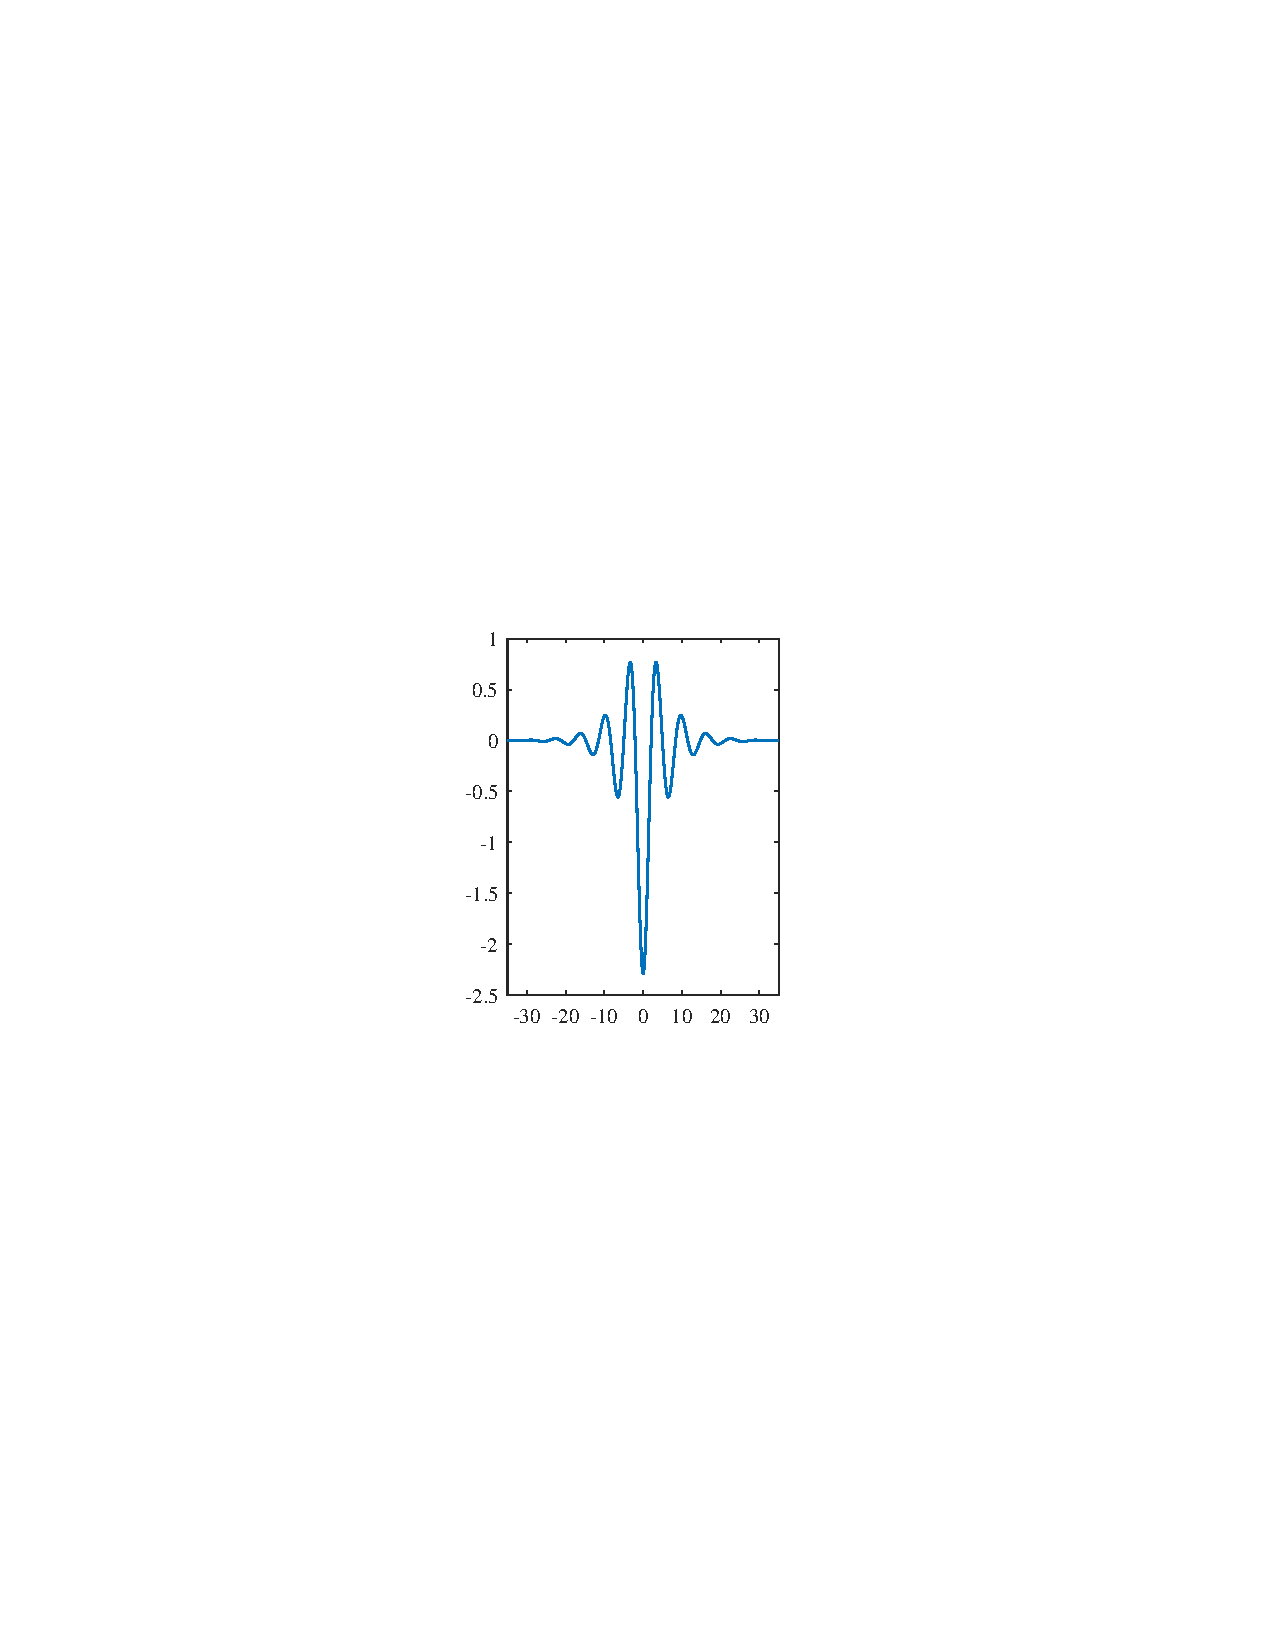
\includegraphics{images/other/single1354}&
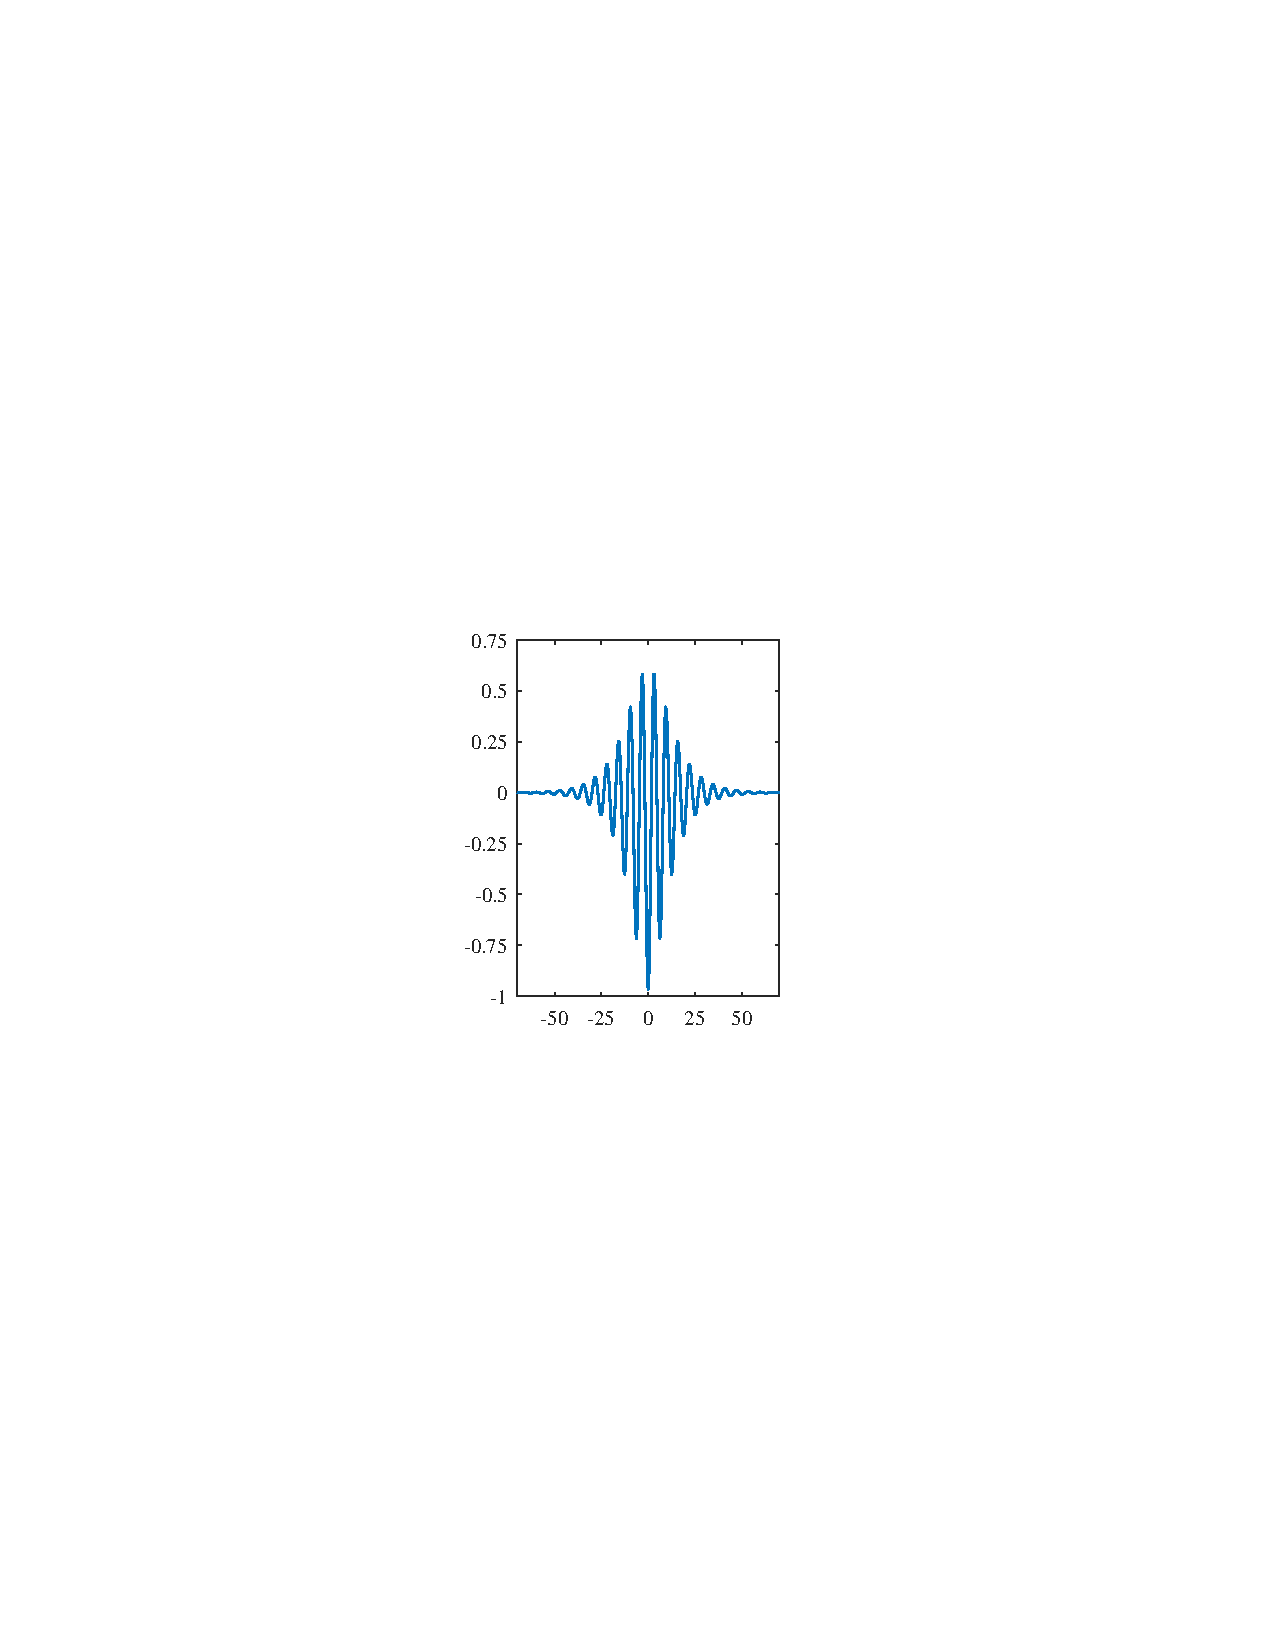
\includegraphics{images/other/single14} \\
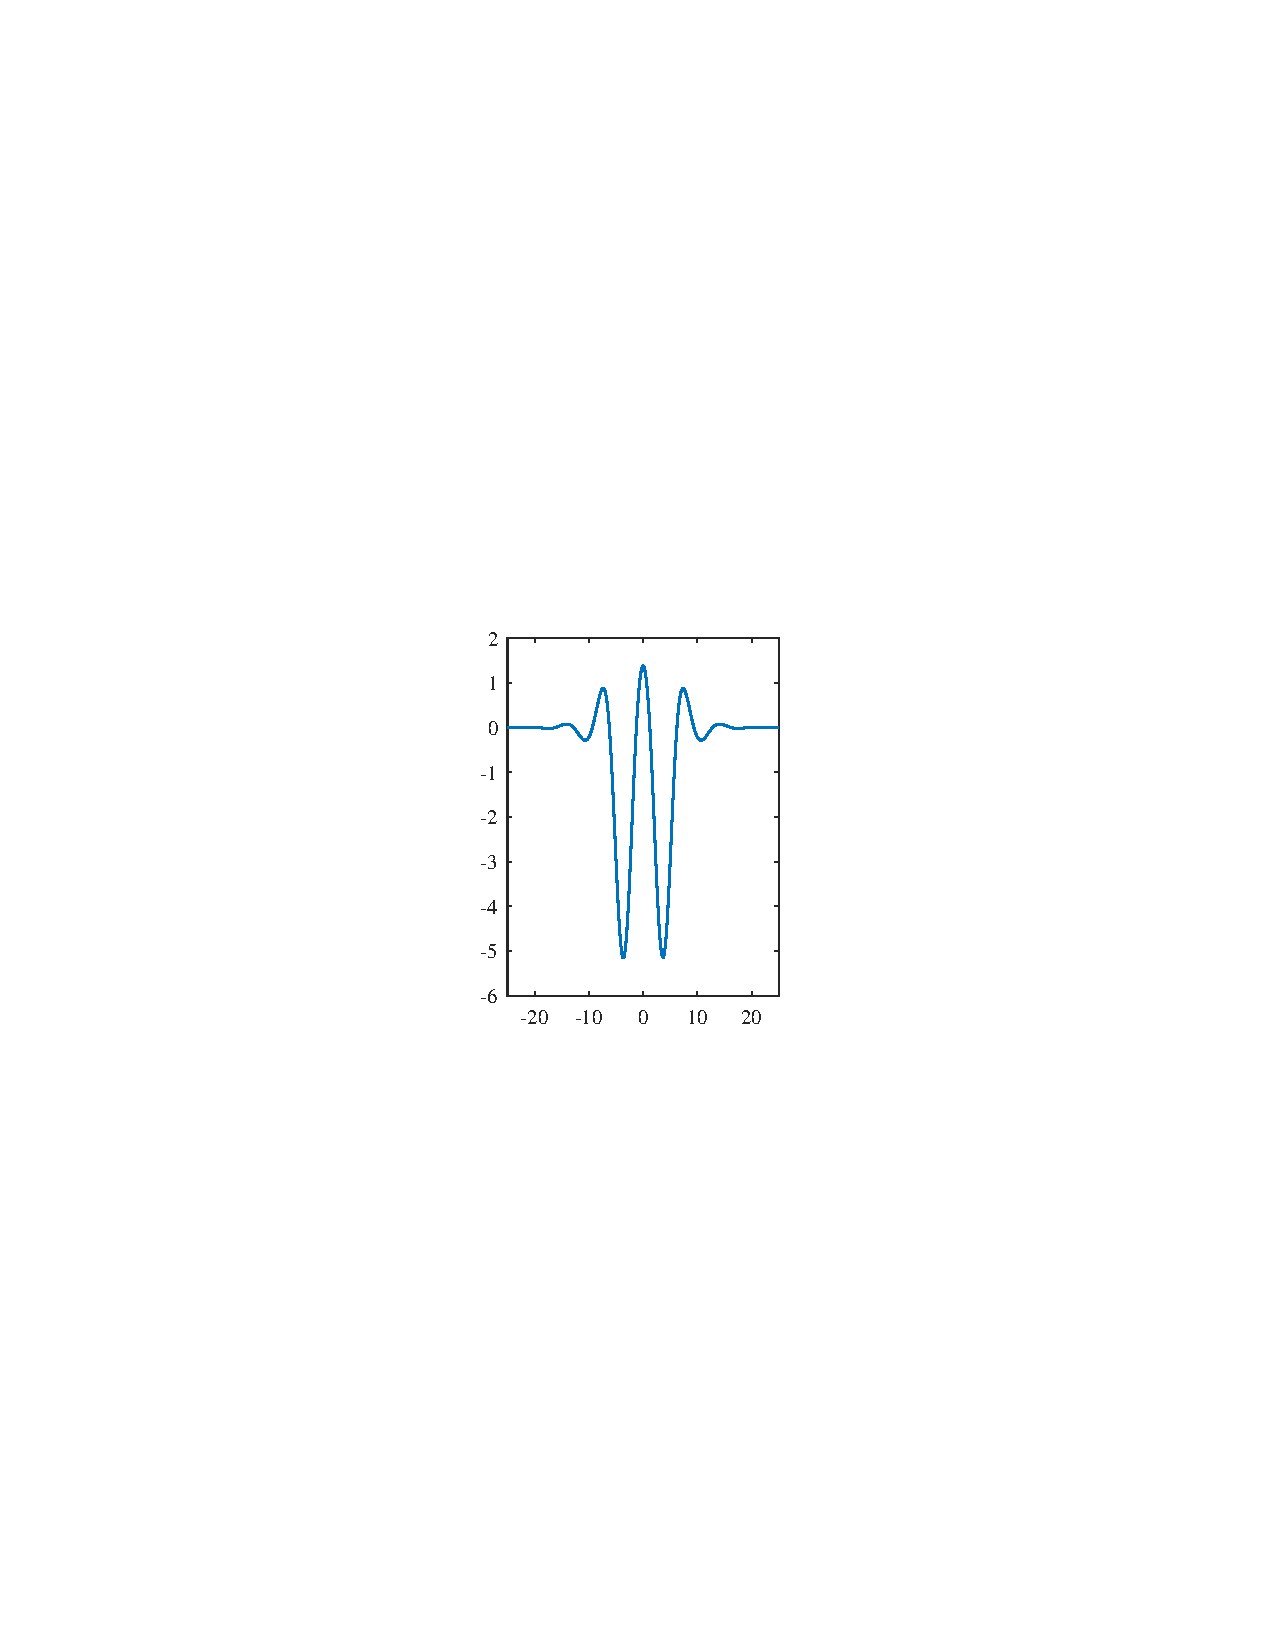
\includegraphics{images/other/double1}&
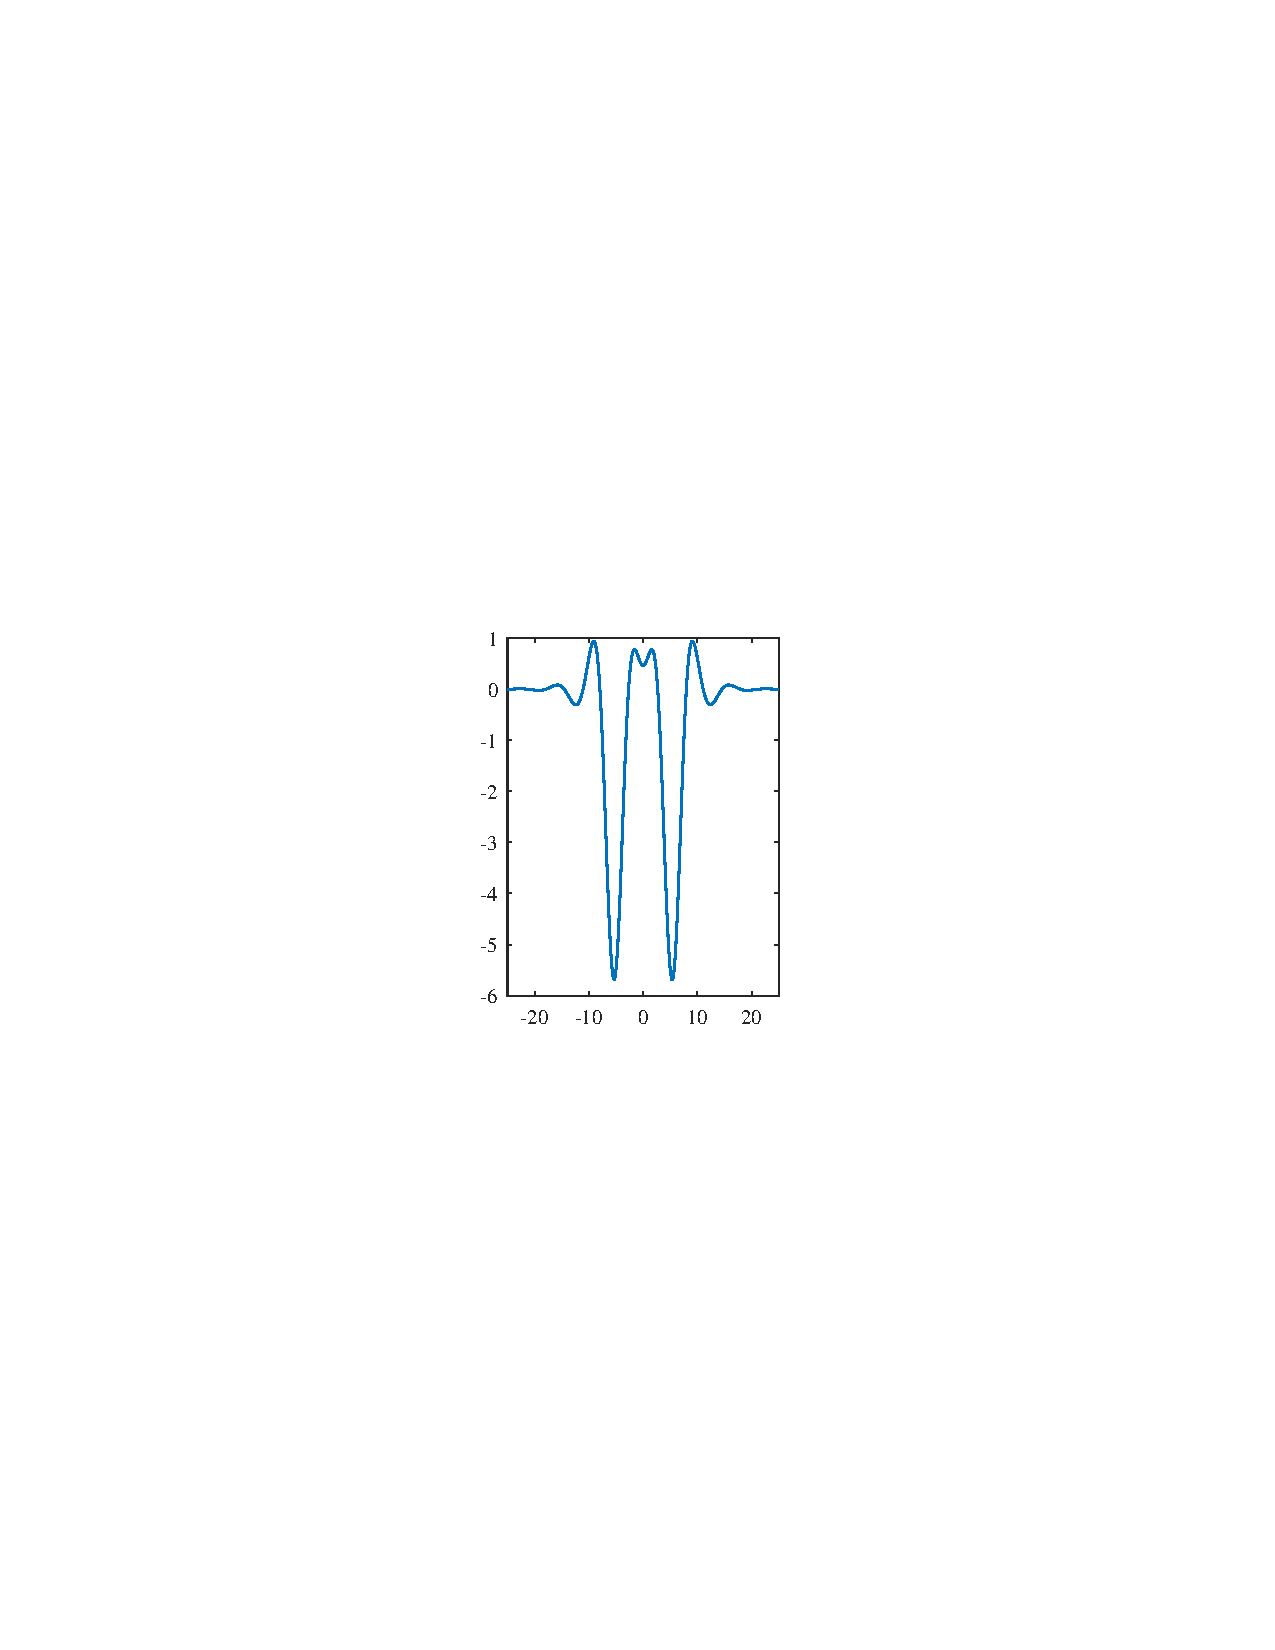
\includegraphics{images/other/double2}
\end{tabular}
\caption[Primary pulse solutions to Chen-McKenna]{Primary pulse solutions $U(x)$ to \cref{suspeq} for $c = 1.354$ (top left) and $c = 1.40$ (top right) constructed using the string method \cite{Chamard2011}. First two double pulse solutions $U_2(x)$ for $c = 1.2$ (bottom) constructed as in \cref{sec:kdv5nummulti}.}
\label{fig:chen1}
\end{figure}

We turn now to the spectral stability of multi-pulse solutions. Linearization of the PDE \cref{suspc} about a multi-pulse solution $U_n$ is the quadratic eigenvalue problem
\begin{equation}\label{quadeig}
\calP_2(\lambda; U_n) = \calI \lambda^2 - 2 c \partial_x \lambda + \calA_0(U_n) = 0,
\end{equation}
where $\calA_0(U_n)$ is defined in \cref{suspA0}. The essential spectrum of \cref{quadeig} is given by
\begin{equation}\label{quadess}
\sigma_{\mathrm{ess}}(\calP_2(\lambda; U_n)) = \sigma_{\mathrm{ess}}(\calT(\lambda)) = \{\rmi r : |r| \geq \rho \},
\end{equation}
where $\rho > 0$ is the minimum of the function $\lambda(r) = c r + \sqrt{1 + r^4}$. The value of $\rho$ is positive for $c \in (0, \sqrt{2})$, and $\rho\to 0$ as $c\to\sqrt{2}$, as shown in \cref{fig:essspecrho}.
\begin{figure}
\centering
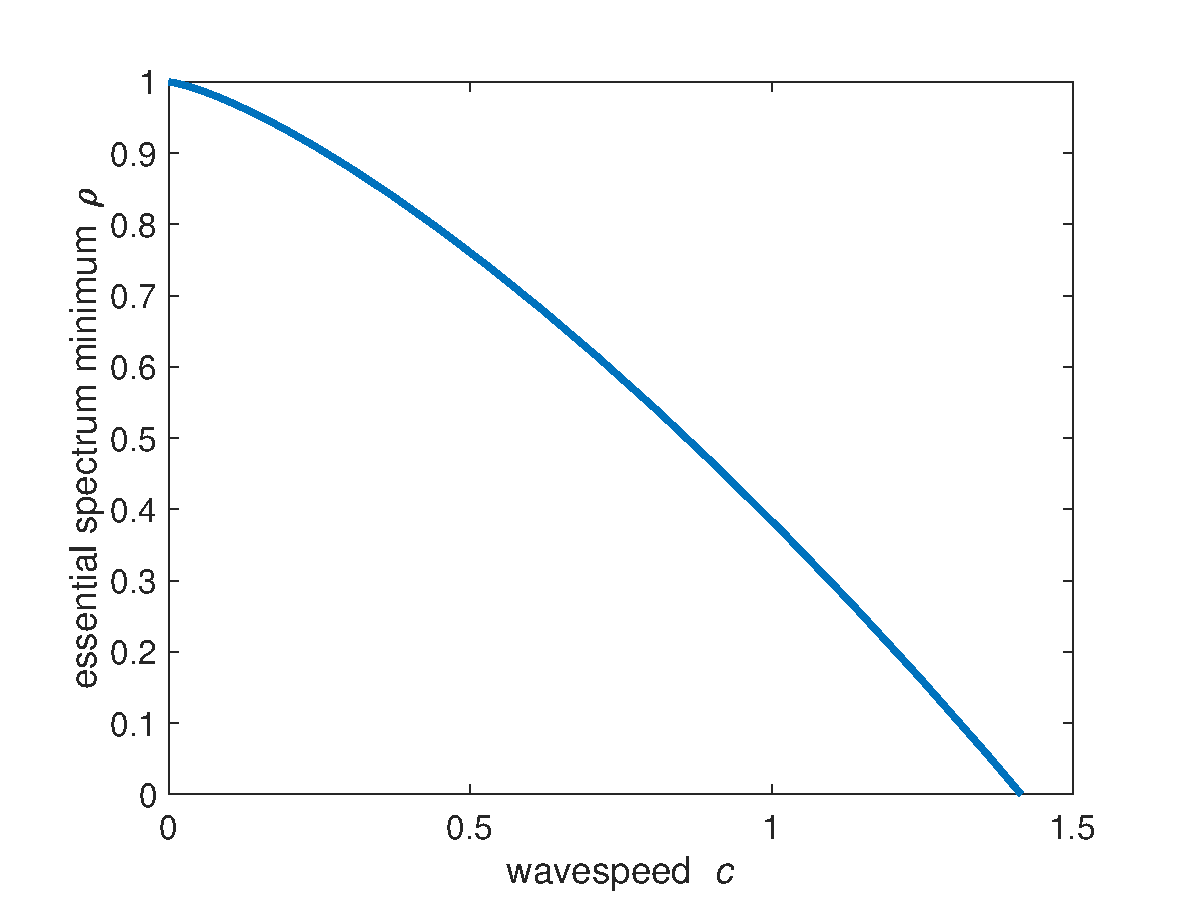
\includegraphics[width=8cm]{images/other/essspecrho.eps}
\caption[Essential spectrum bound for Chen-McKenna]{Minimum of purely imaginary essential spectrum $\rho$ vs. wavespeed $c$.}
\label{fig:essspecrho}
\end{figure}
Since the essential spectrum is purely imaginary and bounded away from 0, spectral stability thus depends entirely on the point spectrum.

For sufficiently well-separated pulses, any imaginary interaction eigenvalues will fall within this gap in the essential spectrum. Thus we avoid the issue we have with KdV5 where interaction eigenvalues may be buried in the essential spectrum. 

To determine the point spectrum, we can adapt the method in \cite{Sandstede1998} as we did in \cref{chapter:kdv5homoclinic}. Since the rest state is hyperbolic, we do not need the exponential weight. Rather than do that, in \cite{kapitula2019} we determine the spectrum using a reformulation of the Krein matrix which can be used for quadratic eigenvalue problems such as \cref{quadeig}.  Briefly, the Krein matrix is meromorphic, matrix-valued function $\vK(\lambda)$ associated with an eigenvalue problem with the property that $\det\vK(\lambda)=0$ only if $\lambda$ is a polynomial eigenvalue \cite[Theorem 3.1]{kapitula2019}. Furthermore, the Krein matrix can be used to determine the Krein signature of a purely imaginary eigenvalue. To obtain the Krein matrix, we project \cref{quadeig} onto a finite-dimensional subspace. For this problem, we choose the space $S$, which defined above after \cref{suspA0}.

In \cite[Theorem 6.8]{kapitula2019}, we prove that for an $n$-pulse solution $U_n$, the Krein matrix associated with \cref{quadeig} is diagonally dominant, thus we can determine the interaction eigenvalues from the diagonal entries of the Krein matrix. In addition, we use the Hamiltonian-Krein index, a tool which counts the potentially unstable eigenvalues, to conclude that this method locates all of the potentially unstable eigenvalues. The main result is summarized in the following theorem, which adapts \cite[Corollary 6.9]{kapitula2019} to the notation used in previous chapters.

\begin{theorem}\label{chenstab}
Assume \cref{chenhyp}. For $c \in (0, \sqrt{2})$, let $U(x)$ be the primary pulse solution, and let $d''(c)$ be defined as in \cref{dcc}. Let $(m_1, \dots, m_{n-1})$ be a homoclinic parameterization, and let $r_*$ be as in Theorem \ref{multipulseexistR}. For $r \in \mathcal{R}$ with $r \leq r_*$, let $U_n(x)$ be an $n-$pulse solution to \cref{suspeq}. Let $\{\mu_1, \dots, \mu_{n-1}, 0\}$ be eigenvalues of $\calA_0(U_n)$ which are close to 0. Then there are $(n-1)$ pairs of interaction eigenvalues of \cref{quadeig} which are close to 0. These are described as follows. For each $j=1,2,\dots,n-1$,
\begin{enumerate}
  \item if $m_j$ is odd (equivalently, $\mu_j<0$), there is a corresponding pair of purely imaginary interaction eigenvalues,
  \begin{equation}\label{npulseKreineigs}
	\lambda_j^\pm = \pm \rmi \left( \|\partial_xU\| \sqrt{ \frac{|\mu_j|}{d''(c)} } + \mathcal{O}(r^{3/2}) \right),
	\end{equation}
  each of which has negative Krein signature
  \item if $m_j$ is even (equivalently, $\mu_j>0$), there is a corresponding pair of real interaction eigenvalues,
   	\[
	\lambda_j = \pm \left( \|\partial_xU\| \sqrt{ \frac{\mu_j}{d''(c)} } + \mathcal{O}(r^{3/2}) \right).
	\]
  In particular, there exists a positive, real eigenvalue.
\end{enumerate}
In addition, there is a geometrically simple eigenvalue at $\lambda=0$ with corresponding eigenfunction $\partial_x U_n$. All other point spectra is purely imaginary, and has positive Krein signature.
\end{theorem}

\begin{remark}
If all the small, nonzero eigenvalues $\{ \mu_1, \dots, \mu_{n-1} \}$ of $\calA_0(U_n)$ are negative, and if the individual pulses are sufficiently well-separated, then the $n$-pulse is spectrally stable; otherwise, it is unstable.
\end{remark}

Numerical analysis supporting the results of \cref{chenstab} is shown in \cref{fig:quadeigdouble}. Note that the essential spectrum is bounded away from 0, which provides ``empty space'' for the interaction eigenvalues to occupy. The essential spectrum consists of discrete points due to the discretization of the differential operators. Finally, although we have characterized the spectrum of multi-pulse solutions to Chen-McKenna, we would like to know what this implies for nonlinear stability of these solutions. In particular, what does this imply physically for traveling waves on a suspension bridge? This is discussed briefly in \cref{sec:concChen}.
\begin{figure}
\centering
\begin{tabular}{cc}
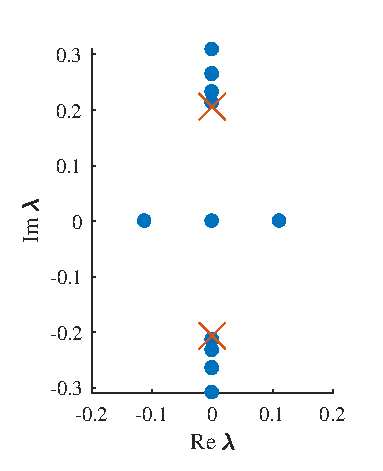
\includegraphics[width=5cm]{images/other/spec12_double1}&
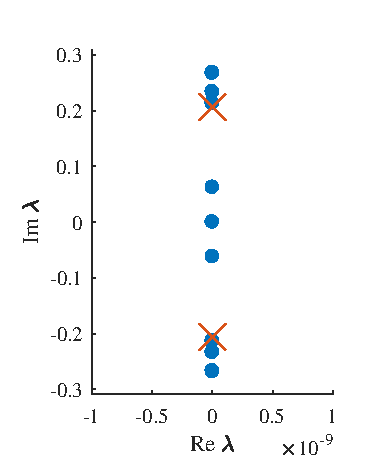
\includegraphics[width=5cm]{images/other/spec12_double2}
\end{tabular} 
\caption[Eigenvalues for double pulses in Chen-McKenna]{Eigenvalues of \cref{quadeig} for double pulses 0 (left) and 1 (right) for $c=1.2$. The edge of the essential spectrum is marked with a (red) cross. For the right panel the two purely imaginary polynomial eigenvalues nearest the origin have negative Krein signature. Finite difference methods with $N = 512$ and periodic boundary conditions.}
\label{fig:quadeigdouble}
\end{figure}

\section{Discrete nonlinear Schr{\"o}dinger equation}\label{sec:DNLS}

The discrete nonlinear Schr{\"o}dinger equation (DNLS) is the 
\begin{equation}\label{DNLS}
i\dot{\psi}_n + d(\psi_{n+1} - 2 \psi_n + \psi_{n-1}) + |\psi_n|^2 \psi_n = 0,
\end{equation}
which is (2.12) in \cite{Kevrekidis2009}, where we have taken $\beta = -1$ and $\sigma = 1$. The parameter $d$ represents the coupling between nodes; $d > 0$ is the focusing case, and $d < 0$ the defocusing case~\cite{Kevrekidis2009}. Equation \cref{DNLS} is Hamiltonian, with energy given by (2.17) in \cite{Kevrekidis2009,pelinovsky_2011}. Of general interest is the existence and stability of standing waves, which are bound state solutions of the form $\psi_n(t) = e^{i \omega t}\phi_n$~\cite{alfimov}. Making this substitution in \cref{DNLS} and simplifying, a standing wave solves the steady state equation
\begin{equation}\label{DNLSequilib}
d(\phi_{n+1} - 2 \phi_n + \phi_{n-1}) - \omega \phi_n + |\phi_n|^2 u_n = 0.
\end{equation}

In contrast to the continuous NLS equation, the discrete NLS equation is not translation invariant. There are only two stationary soliton solutions (modulo shifting the entire solution by an integer number of lattice points): an on-site soliton, centered on a single lattice point, and an off-site soliton, centered between two lattice points. These are shown in the left panels of \cref{fig:DNLSsingle}
\begin{figure}
\centering
\begin{tabular}{cc}
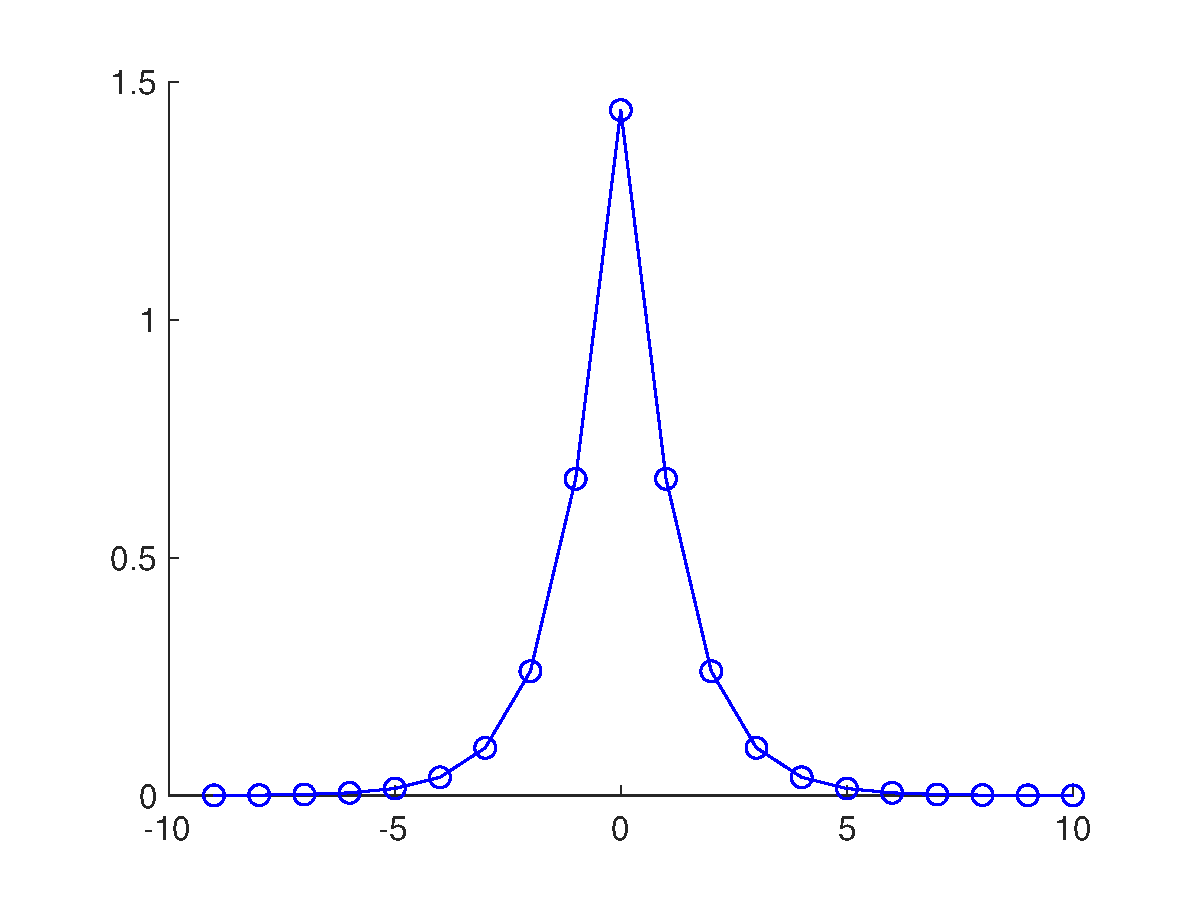
\includegraphics[width=5cm]{images/other/onsite}&
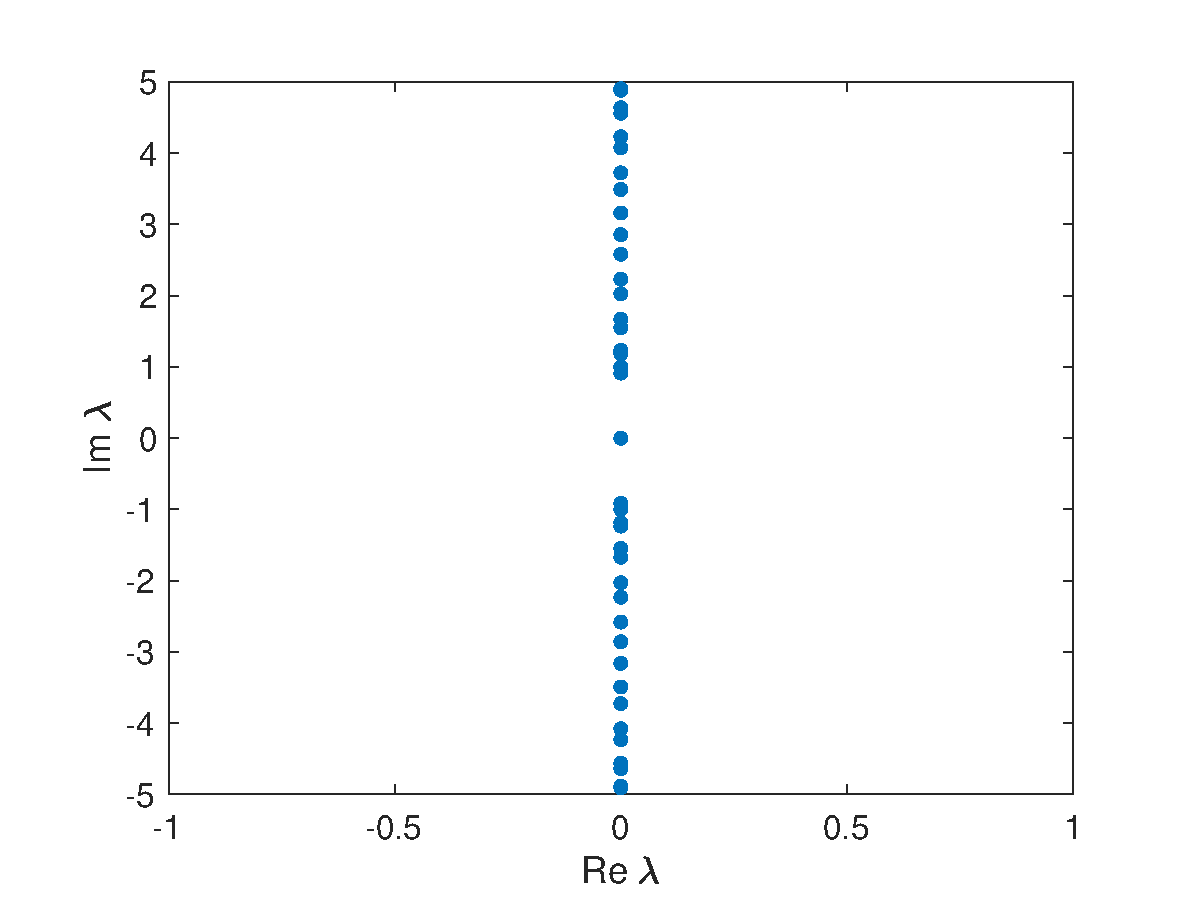
\includegraphics[width=5cm]{images/other/onsitespec} \\
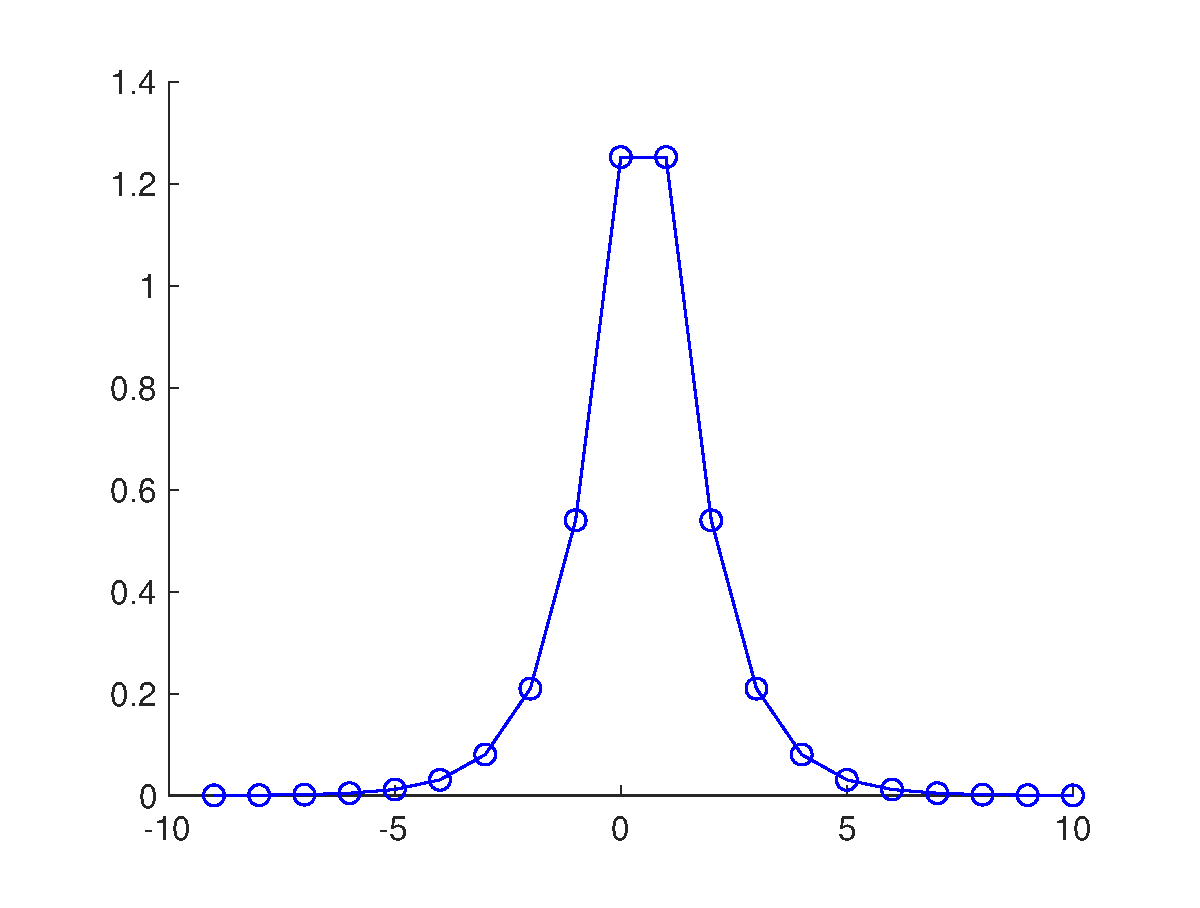
\includegraphics[width=5cm]{images/other/intersite}&
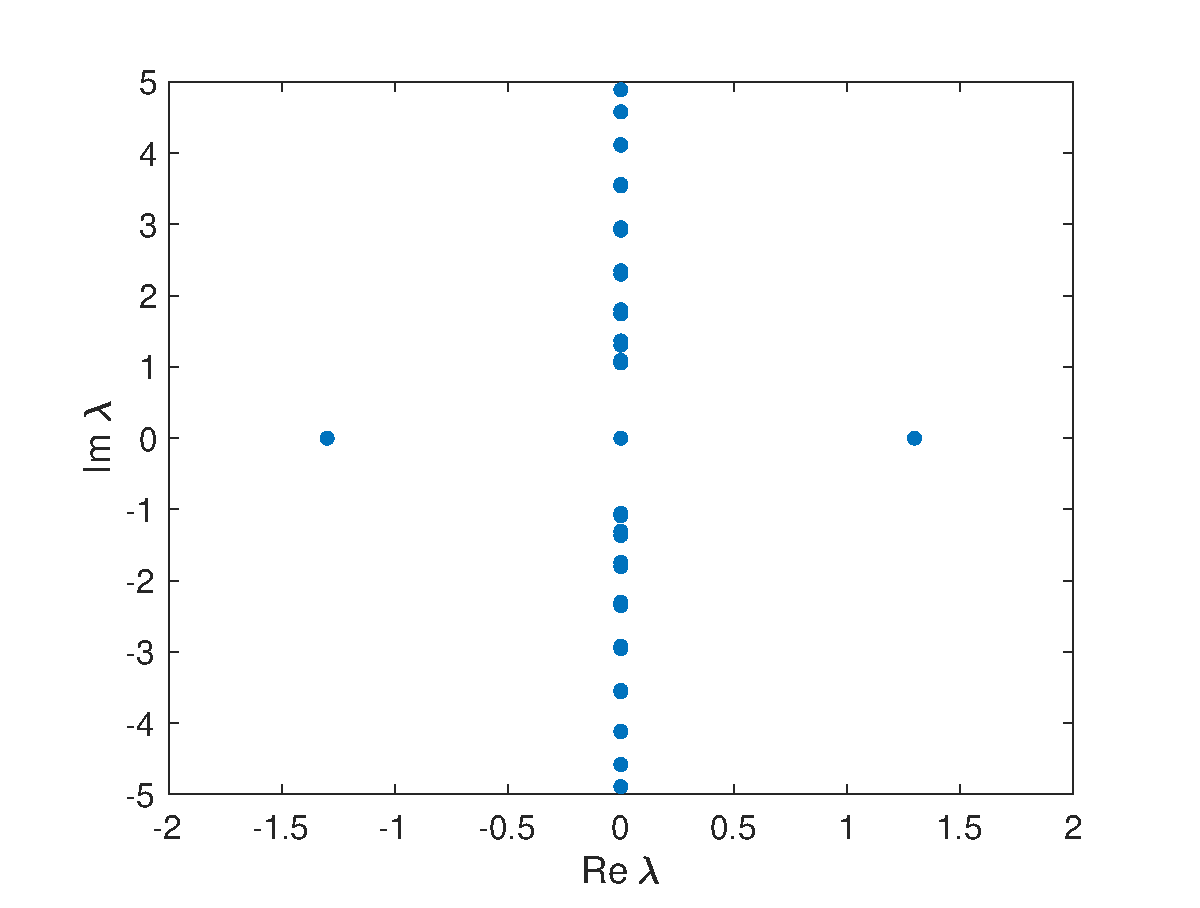
\includegraphics[width=5cm]{images/other/intersitespec}
\end{tabular}
\caption[On-site and inter-site solitons for DNLS]{Two distinct soliton solution for DNLS together with the spectrum of the linearization about the solutions. On-site soliton (top) and inter-site soliton (bottom). Discretization with 20 lattice points, $d = 1$, $\omega = 1$.}
\label{fig:DNLSsingle}
\end{figure}
The spectra of the linearization about the two soliton solutions is shown in the right panels of \cref{fig:DNLSsingle}. Since the off-site soliton is spectrally unstable, we will only consider the on-site soliton from here on. From~\cite{herrmann_2011}, a symmetric, real-valued, on-site soliton solution $q_n$ exists to \cref{DNLSequilib} for all $\omega \neq 0$ and $d \geq 0$. This solution $q_n$ furthermore is differentiable in $\omega$. 

If $\phi_n$ is a solution to \cref{DNLSequilib}, then by rotational symmetry it is not hard to show that $e^{i \theta} \phi_n$ is also a solution. An $m$-pulse solution is composed of $m$ individual copies of the primary pulse $q_n$ glued together. Each copy of $q_n$ is associated with a phase angle $\theta$; since \cref{DNLSequilib} is invariant under rotation, only the differences in phase between consecutive copies of $q_n$ are important. We will characterize an $m-$pulse solution to \cref{DNLSequilib} in terms of the following parameters: 
\begin{enumerate}[(i)]
\item The distances $\{ N_1, \dots, N_{m-1} \}$ in lattice points between consecutive copies of $q_n$.
\item The phase differences $\{ \Delta\theta_1, \dots, \Delta\theta_{m-1} \}$ between consecutive copies of $q_n$.
\end{enumerate}

Before we state our results, we will briefly summarize what is already known about multi-pulse solutions. Many more details can be found in \cite{Kevrekidis2009,pelinovsky_2011}. At the anti-continuum limit ($d = 0$), equation \cref{DNLSequilib} reduces to a system of decoupled algebraic equations. Any $u_n$ with $u_n \in \{ 0, \pm \sqrt{\omega}\}$ is a solution. For sufficiently small $d$, $m$-pulse solutions exist to equation \cref{DNLSequilib} for any pulse distances as long as the phase differences satisfy $\Delta \theta_i \in \{0, \pi\}$ \cite[Proposition 2.1]{Pelinovsky2005}. For sufficiently small $d$, this $m-$pulse is spectrally unstable unless all of the phase differences $\Delta \theta_i$ are $\pi$; in that case there are $m-1$ pairs of purely imaginary eigenvalues with negative Krein signature \cite[Theorem 3.6]{Pelinovsky2005}. This means that these eigendirections, although neutrally stable, are prone to instabilities when parameters (such as $d$) are varied upon collision with other eigenvalues. For any $d$ for which the $m-$pulse exists, if one or more phase differences $\Delta \theta_i$ is 0, it follows from Sturm-Liouville theory that there is at least one positive, real eigenvalue \cite{Kapitula2001a}.

We use Lin's method to extend these results to regimes further from the anti-continuum limit. In effect, we are replacing the condition that $d$ is sufficiently small with the condition that the individual pulses are well separated. We have the following theorem regarding the existence of $m-$pulse solutions. For notational simplicity, we will write solutions to \cref{DNLSequilib} as $u(n)$ rather than $u_n$ as is traditional in the literature. Specifically, the primary pulse solution will be written as $q(n)$.

\begin{theorem}\label{DNLSexisttheorem}
There exists a positive integer $N_0$ (which depends on $\omega$ and $d$), with the following property. For any $m \geq 2$, pulse distances $N_i \geq N_0$, and phase differences $\Delta\theta_i \in \{0, \pi\}$, there exists a unique $m-$pulse solution $q_m(n)$ to \cref{DNLSequilib} which resembles $m$ consecutive copies of the on-site pulse $q(n)$. No other phase differences are possible.
\end{theorem}

The linearization about $q_m(n)$ has a kernel with algebraic multiplicity 2 and geometric multiplicity 1 which is a result of rotational invariance. The following theorem locates the small eigenvalues of the linearization about $q_m(n)$ resulting from interaction between consecutive copies of $q(n)$. 

\begin{theorem}\label{DNLSeigtheorem}
Let $q_m(n)$ be an $m-$pulse solution to \cref{DNLSequilib} with pulse distances $N_i$ and phase differences $\Delta\theta_i$. Assume that $M > 0$, where
\[
M = \sum_{n=-\infty}^\infty q(n) \partial_\omega q(n) = \partial_\omega \left( \frac{1}{2} \sum_{n=-\infty}^\infty q(n)^2 \right).
\]
Let $N = \frac{1}{2} \min\{ N_1, \dots, N_{m-1}\}$. Then for $N$ sufficiently large, there exist $m-1$ pairs of interaction eigenvalues $\{\pm \lambda_1, \dots, \pm \lambda_{m-1}\}$, which can be grouped as follows. There are $k_\pi$ pairs of purely imaginary eigenvalues and $k_0$ pairs of real eigenvalues, where $k_\pi$ is the number of phase differences $\Delta\theta_i$ which are $\pi$, and $k_0$ is the number of phase differences $\Delta\theta_i$ which are $0$. The $\lambda_j$ are close to 0 and are given by the following formula
\begin{align}\label{eigsDNLS}
\lambda_j &= \sqrt{\frac{d \mu_j}{M}} + \mathcal{O}(r^{-2N}) && j = 1, \dots, m-1,
\end{align}
where
\begin{align}\label{eigr}
r = 1 + \frac{\omega}{2 d} \left( 1 + \sqrt{1 + \frac{4 d}{\omega}} \right),
\end{align}
$d$ is the coupling constant and $\{ \mu_1, \dots, \mu_{m-1} \}$ are the distinct, real, nonzero eigenvalues of the symmetric, tridiagonal matrix
\begin{align}\label{DNLSmatrixA}
A &= \begin{pmatrix}
-\cos(\Delta\theta_1) b_1 & \cos(\Delta\theta_1) b_1 & & &  \\
\cos(\Delta\theta_1) b_1 & -\cos(\Delta\theta_1) b_1 - \cos(\Delta\theta_2) b_2 & \cos(\Delta\theta_2) b_2 \\
& \ddots & \ddots \\
& &  \cos(\Delta\theta_{m-1}) b_{m-1} & -\cos(\Delta\theta_{m-1}) b_{m-1}  \\
\end{pmatrix},
\end{align}
where
\begin{align}\label{bieq}
b_i = \begin{cases}
q\left(\frac{N_i}{2}\right) \left[ q\left(\frac{N_i}{2} + 1\right) - q\left(\frac{N_i}{2} - 1\right) \right] & N_i \text{ even} \\
q\left(\frac{N_i-1}{2}\right)\left(\frac{N_i+3}{2}\right) 
- \left(\frac{N_i+1}{2}\right)q\left(\frac{N_i-3}{2}\right) & N_i \text{ odd}
\end{cases} \:.
\end{align}
\end{theorem}

\begin{remark}
There is strong numerical evidence that $M > 0$, i.e. the Melnikov condition is satisfied.
\end{remark}

\begin{remark}
If all the nonzero eigenvalues $\mu_j$ of $A$ are larger than $\mathcal{O}(r^{-4N})$, then the formula \cref{eigsDNLS} is the sum of a leading order term and a small remainder term. A good approximation for the eigenvalues $\lambda_j$ can be obtained by computing the eigenvalues of $A$. A sufficient condition for this is $N_{\mathrm{max}} < 2 N$, where $N_{\mathrm{max}} = \frac{1}{2} \max\{ N_1, \dots, N_{m-1}\}$.
\end{remark}

\noindent In addition, we remark that if $b_1 = \dots = b_{m-1} = b$, $A = -b \mathcal{M}_1$, where the matrix $\mathcal{M}_1$ is defined in \cite[(2.84)]{Kevrekidis2009} and represents interactions between neighboring sites.

We can compute the nonzero eigenvalues of \cref{DNLSmatrixA} in several special cases. In the first corollary, we consider the case where the pulse distances $N_i$ are equal.

\begin{corollary}\label{DNLSeigcorr}Let $q_m(n)$ be an $m-$pulse solution to \cref{DNLSequilib} with pulse distances $N_i = 2N$ and phase differences $\Delta\theta_i$. Then the $\lambda_j$ are as follows.
\begin{enumerate}[(i)]
\item For $m = 2$, we have
\begin{align}\label{2pulseeigs}
\lambda_1 &= 
\begin{cases}
\sqrt{2}\nu  + \mathcal{O}(r^{-2N}) & \Delta\theta_1 = 0 \\
\sqrt{2}\nu i + \mathcal{O}(r^{-2N}) & \Delta\theta_1 = \pi
\end{cases} \:.
\end{align}
\item For $m = 3$, we have
\begin{align}\label{3pulseequaleigs}
\lambda_{1, 2} &= \begin{cases}
\nu, \sqrt{3} \nu + \mathcal{O}(r^{-2N}) & (\Delta\theta_1, \Delta\theta_2) = (0, 0) \\
3^{1/4}\nu, 3^{1/4}\nu i + \mathcal{O}(r^{-2N}) & (\Delta\theta_1, \Delta\theta_2) = (0, \pi) \\
\nu i, \sqrt{3} \nu i + \mathcal{O}(r^{-2N}) & (\Delta\theta_1, \Delta\theta_2) = (\pi, \pi)
\end{cases}\:.
\end{align}
\item For $m > 3$, if $\Delta\theta_i = \Delta\theta$ for all $i$,
\begin{align*}
\lambda_j = \begin{cases}
\sqrt{2\left( \cos\frac{\pi j}{m} - 1 \right)}\nu + \mathcal{O}(r^{-2N}) & \Delta\theta = 0 \\
\sqrt{2\left( \cos\frac{\pi j}{m} - 1 \right)}\nu i + \mathcal{O}(r^{-2N}) & \Delta\theta = \pi
\end{cases}
\end{align*}
for $j = 1, \dots, m-1$.
\end{enumerate}
where $\nu = \sqrt{\frac{|b|d}{M}} = \mathcal{O}(r^{-N})$, and $b$ is given by equation \cref{bieq}.
\end{corollary}

In the second corollary, we give a general formula for the eigenvalues for a 3-pulse.

\begin{corollary}\label{DNLSeigcorr2}
Let $q_3(n)$ be an $3-$pulse solution to \cref{DNLSequilib} with pulse distances $N_1, N_2$ and phase differences $\Delta \theta_1, \Delta \theta_2$. Then $\lambda_1, \lambda_2$ are given by
\begin{equation}\label{3pulseeigs}
\begin{aligned}
\lambda_{1,2} = \sqrt{\frac{d}{M}}
&\Big( -b_1\cos\Delta\theta_1 - b_2\cos\Delta\theta_2  \\
&\pm \sqrt{b_1^2 + b_2^2 - b_1 b_2\cos\Delta\theta_1 \cos\Delta\theta_2} \Big)^{1/2} + \mathcal{O}(r^{-2N}).
\end{aligned}
\end{equation}
If $N_1 < N_2 < 2 N_1$, then, to leading order, these have magnitude
\begin{equation}\label{3pulsemag}
\begin{aligned}
|\lambda_1| &= \sqrt{\frac{2 |b_1| d}{M}} = \mathcal{O}(r^{-N_1/2}) \\
|\lambda_2| &= \sqrt{\frac{3 |b_2| d}{2 M}} = \mathcal{O}(r^{-N_2/2}) \:,
\end{aligned}
\end{equation}
where $b_1$ and $b_2$ are given by equation \cref{bieq}.
\end{corollary}

To conclude, we provide numerical verification for these results. We first construct multi-pulse solutions to the steady state DNLS problem by using Matlab for parameter continuation in the coupling constant $d$ from the anti-continuum limit. We then find the eigenvalues of the linearization about this solution using Matlab's \texttt{eig} function. 

First, we look at multi-pulses where the pulse distances are equal.  The left and center panels of \cref{fig:eigendecay1} show the pulse profile and eigenvalue pattern for the two double pulses (of relative phase $0$ and $\pi$). Equation \cref{2pulseeigs} from \cref{DNLSeigcorr} states that for fixed $\omega$ and $d$, the interaction eigenvalues decay as $r^{-N}$. In the right panel of \cref{fig:eigendecay1}, we plot $\log \lambda$ vs. $N$ for the two possible double pulses and construct a least-squares linear regression line. In both cases, the relative error in the slope of this line (which is predicted to be $-\log r$) is order $10^{-4}$. This result provides theoretical and numerical support to the earlier observations of~\cite{Kapitula2001a}.

\begin{figure}
\centering
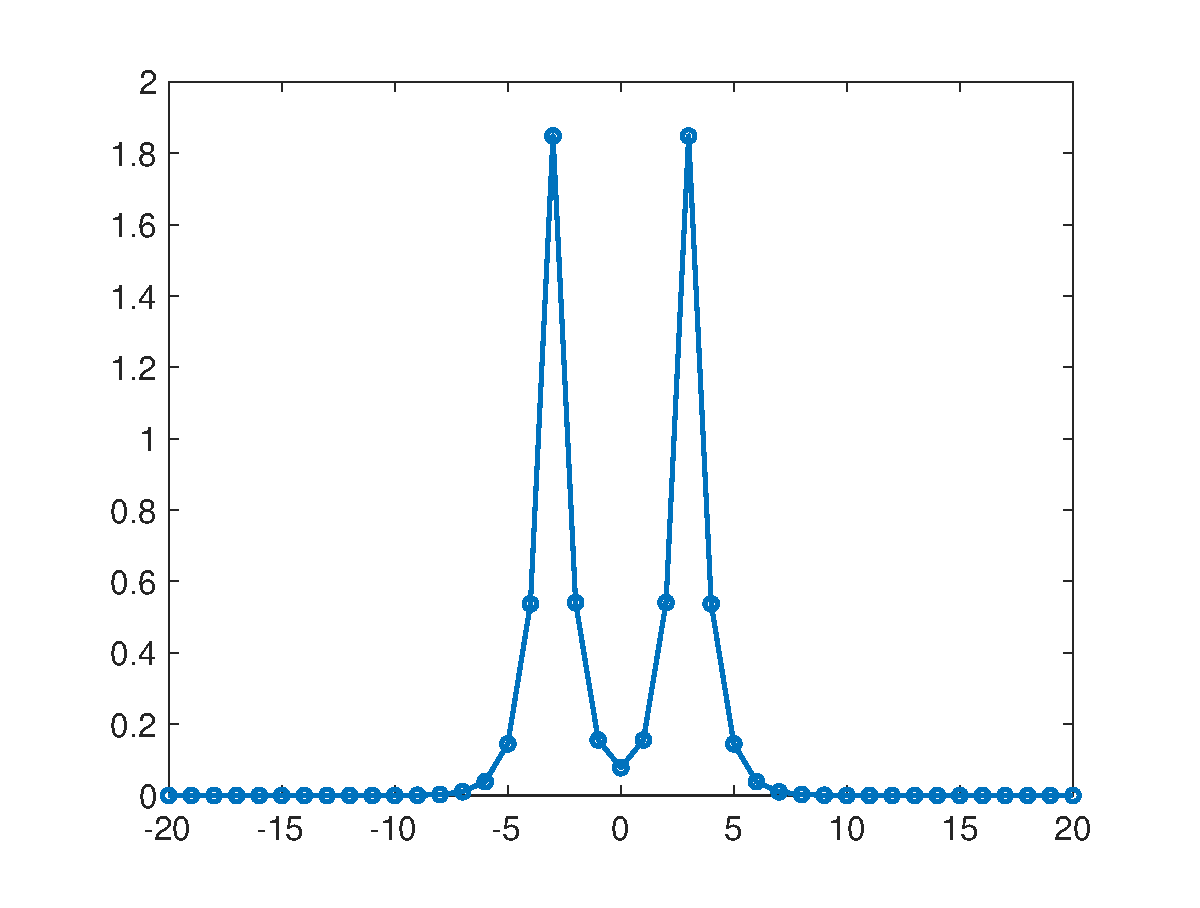
\includegraphics[width=5cm]{images/other/dnlsPP.eps}
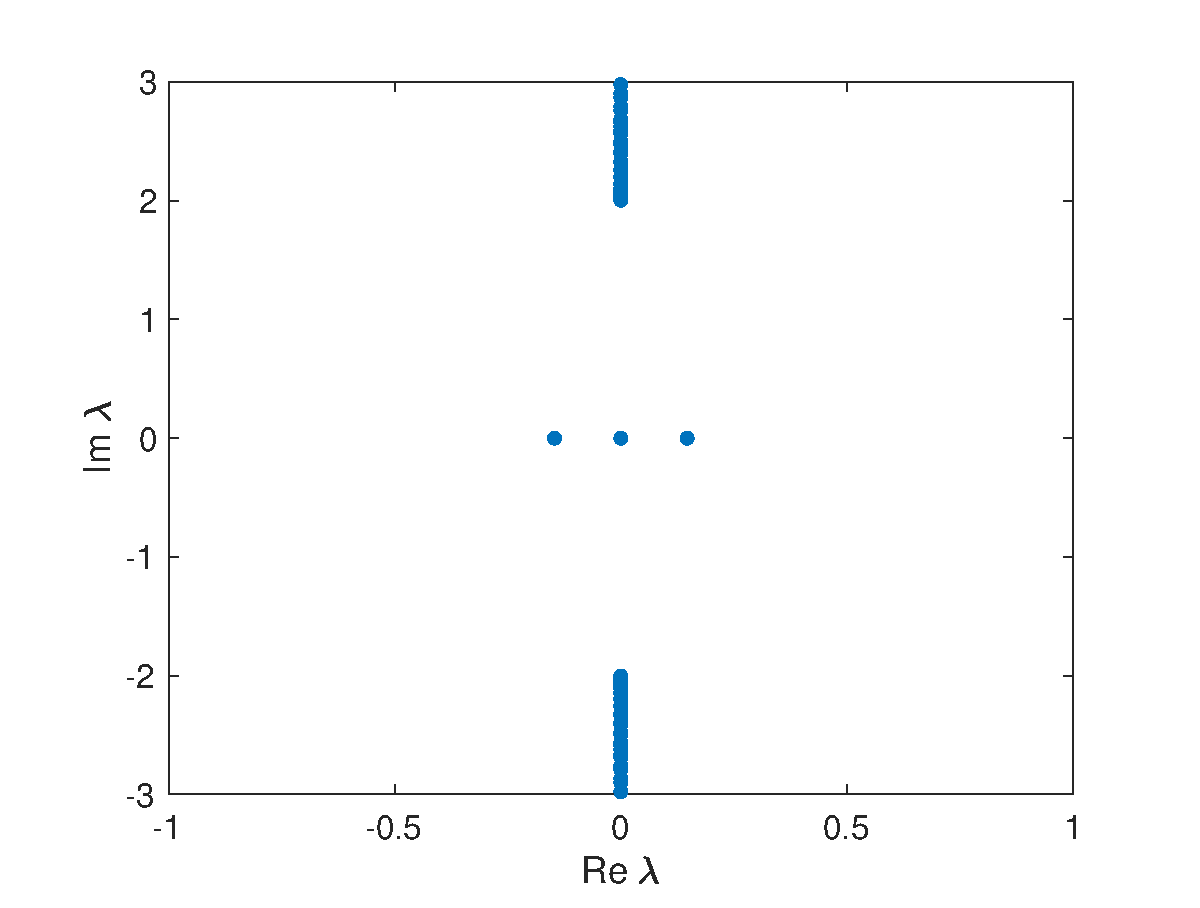
\includegraphics[width=5cm]{images/other/dnlsPPeig.eps}
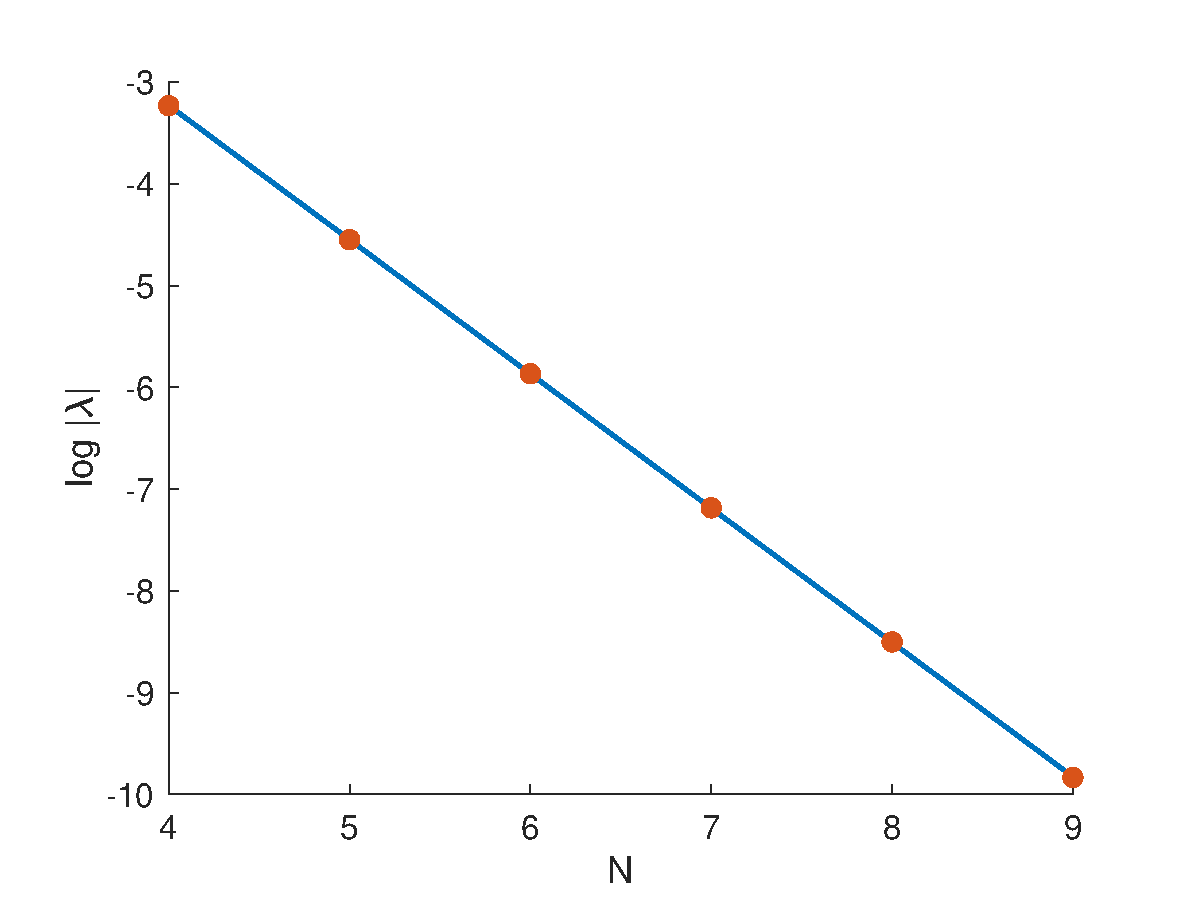
\includegraphics[width=5cm]{images/other/dnlsPPdecay.eps}
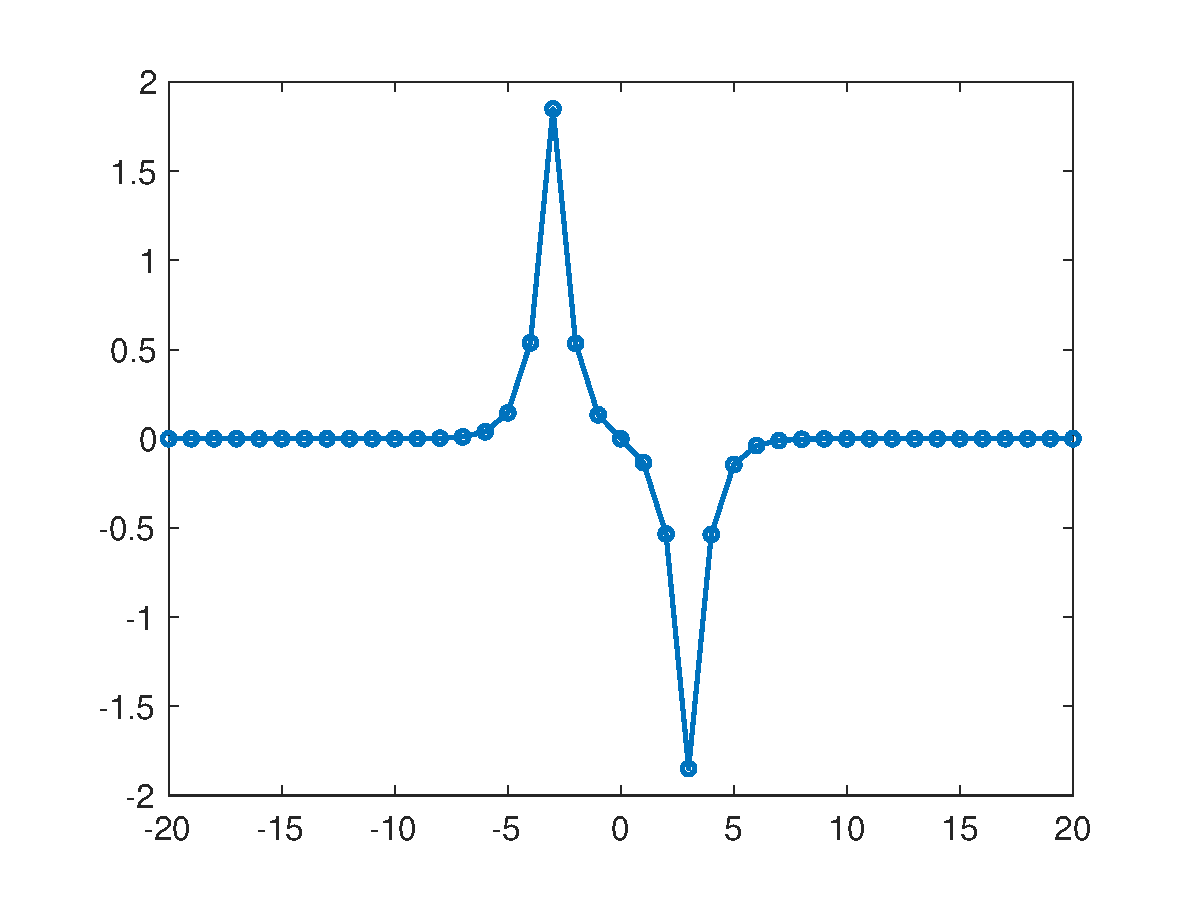
\includegraphics[width=5cm]{images/other/dnlsPM.eps}
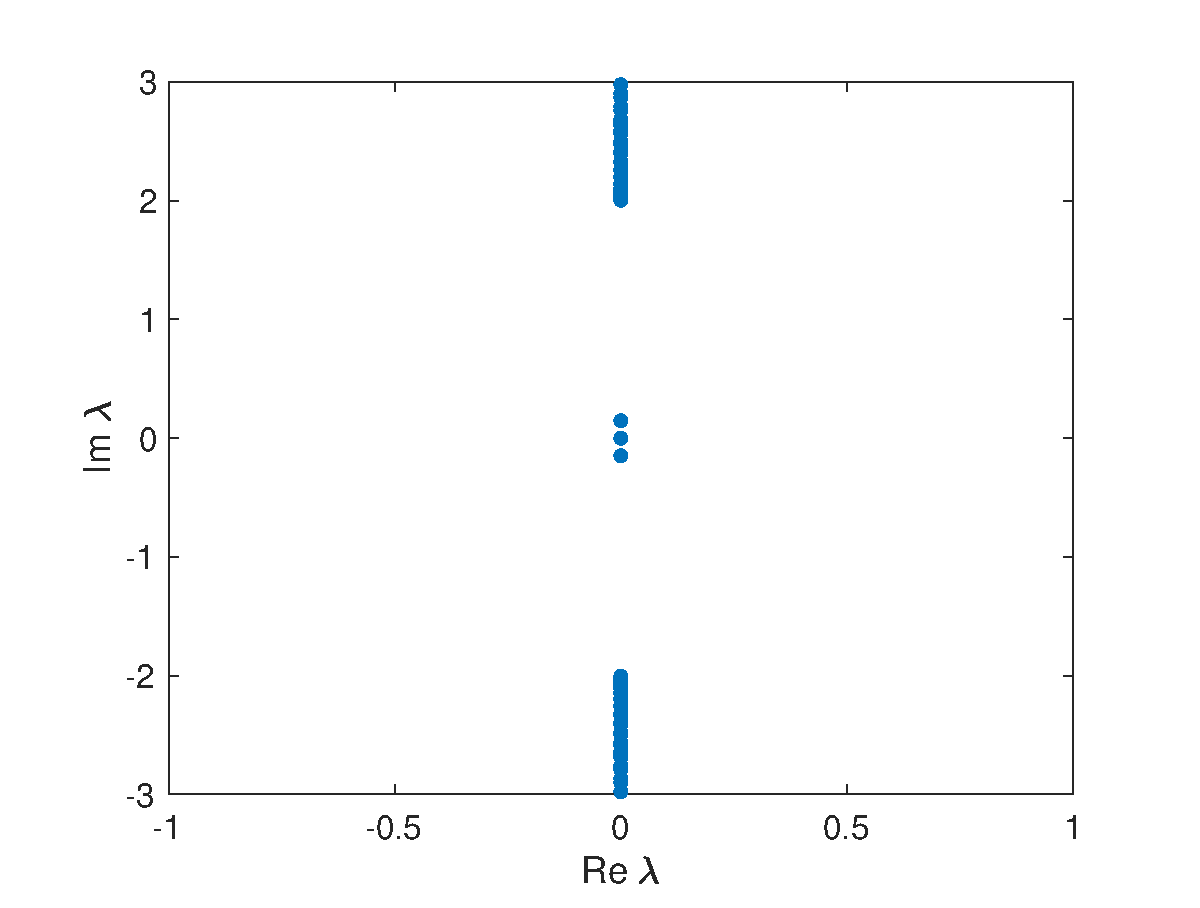
\includegraphics[width=5cm]{images/other/dnlsPMeig.eps}
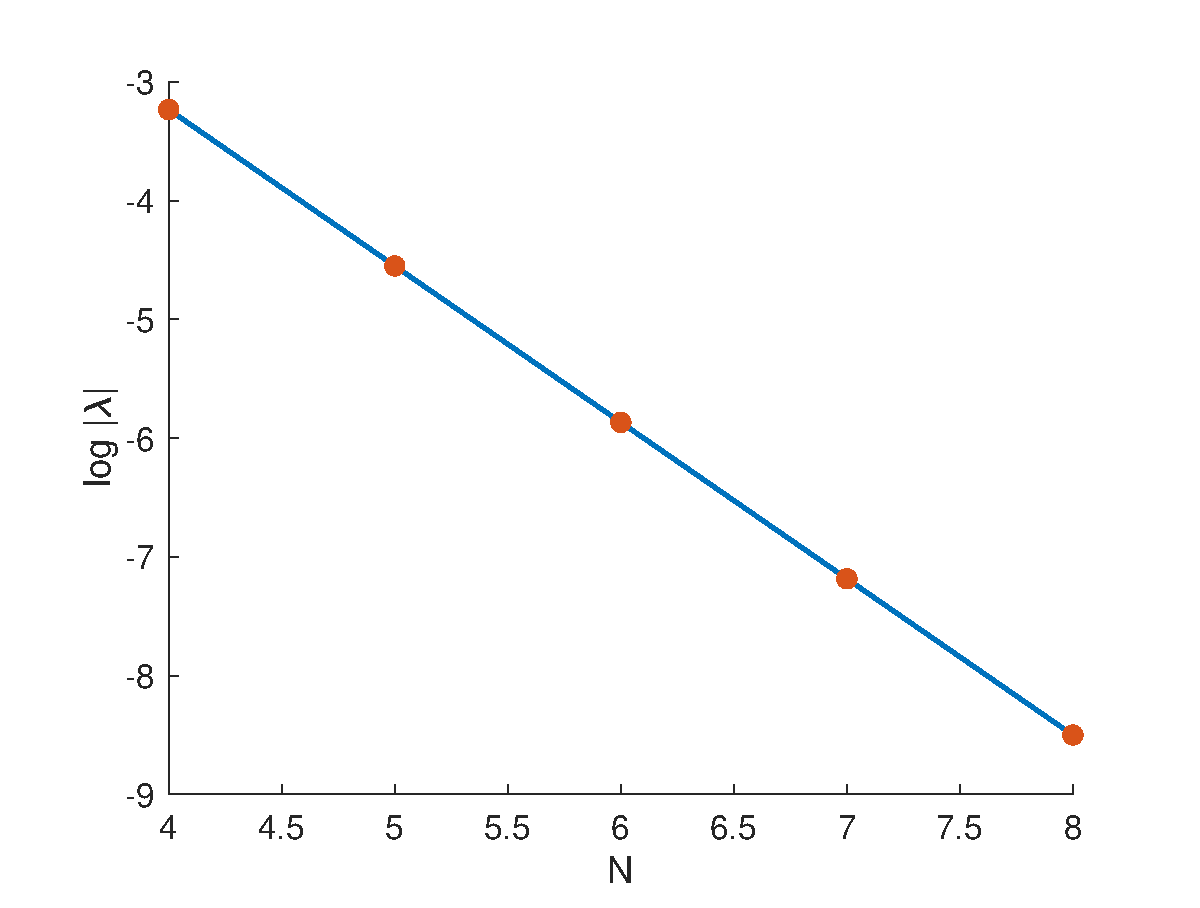
\includegraphics[width=5cm]{images/other/dnlsPMdecay.eps}
\caption[Solutions and eigenvalue patterns for double pulses in DNLS]{Solution profile (left panel), spectral plane eigenvalue pattern (center panel), and plot of $\log(\lambda)$ vs. $N$ with least squares linear regression line (right panel) for $++$ (top) and $+-$ (bottom) pulses. The symbolic notation here and 
below follows that of~\cite{alfimov}, referring
with a symbolic sign representation to the positive
or negative value of the peak of the pulse.
Parameters $\omega = 2$ and $d = 1.0$.}
\label{fig:eigendecay1}
\end{figure}

We do the same for triple pulses with equal pulse distances in \cref{fig:eigendecay2}. Since the pulse distances are equal, both sets of interaction eigenvalues decay as $r^{-N}$ by equation \cref{3pulseequaleigs} from \cref{DNLSeigcorr}. In the right panel of \cref{fig:eigendecay2}, we plot $\log \lambda$ vs. $N$ for the three triple pulses and construct a least-squares linear regression line. In all three cases, 
namely the in-phase (or $+++$) pulse, the 
out-of-phase (or $+-+$) and finally the 
intermediate/mixed phase case
(or $++-$), the relative error of the slope of the least squares linear regression line is of order $10^{-4}$.  

\begin{figure}
\centering
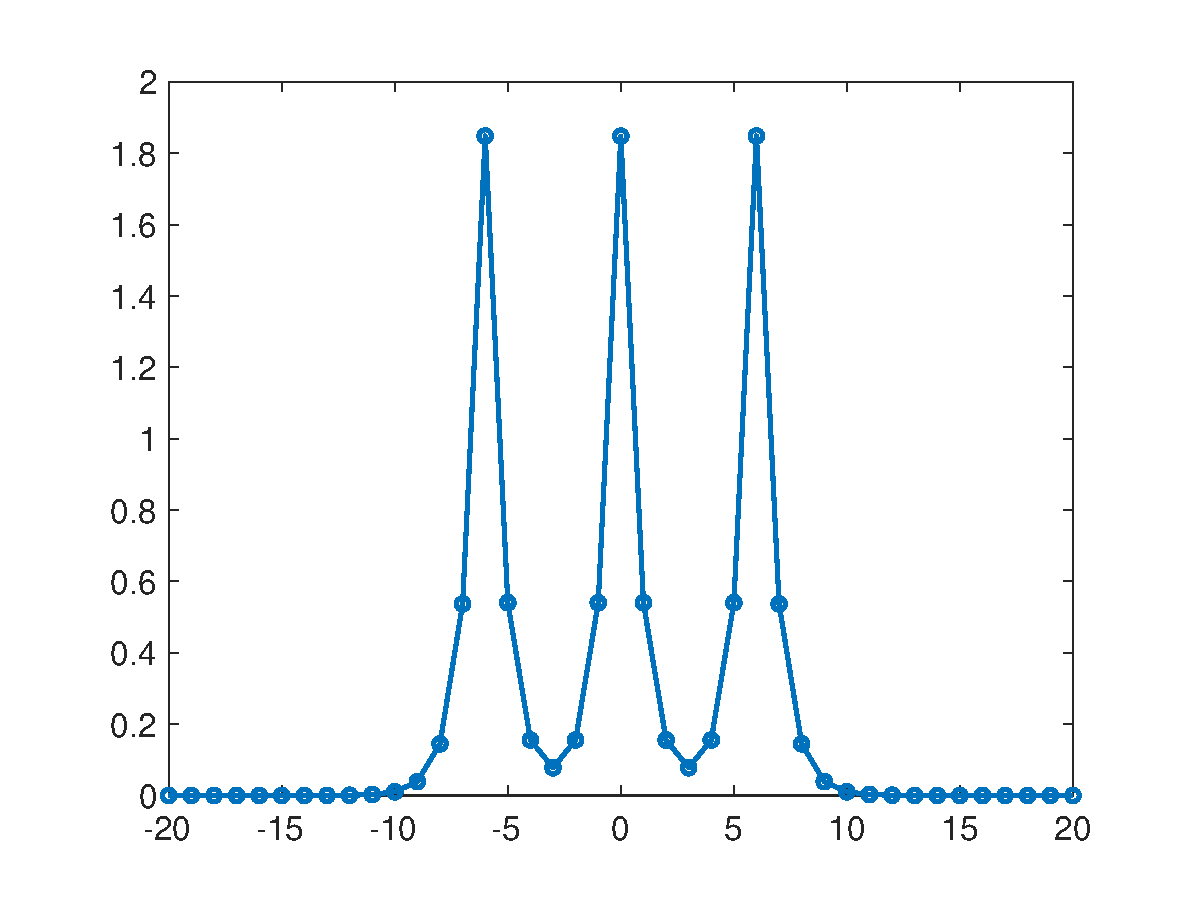
\includegraphics[width=5cm]{images/other/dnlsPPP.eps}
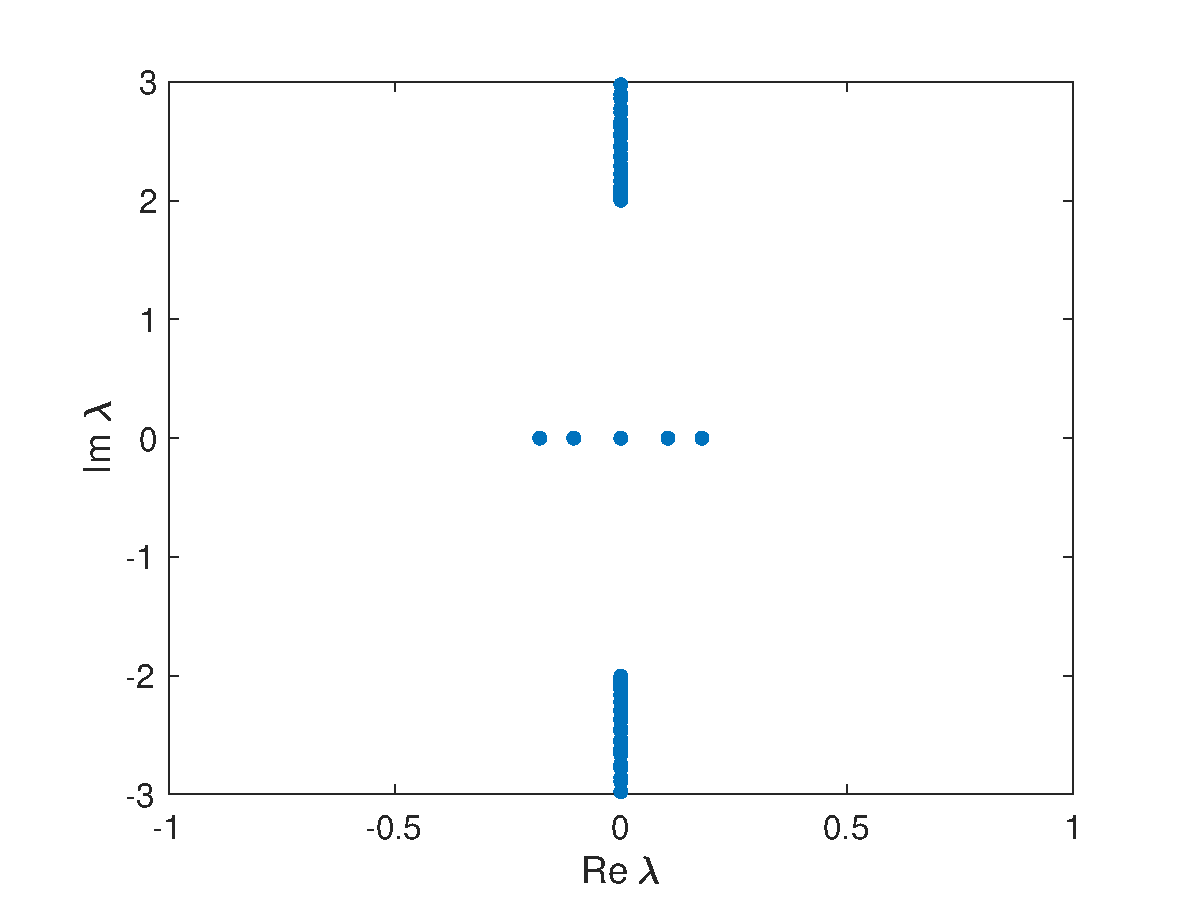
\includegraphics[width=5cm]{images/other/dnlsPPPeig.eps}
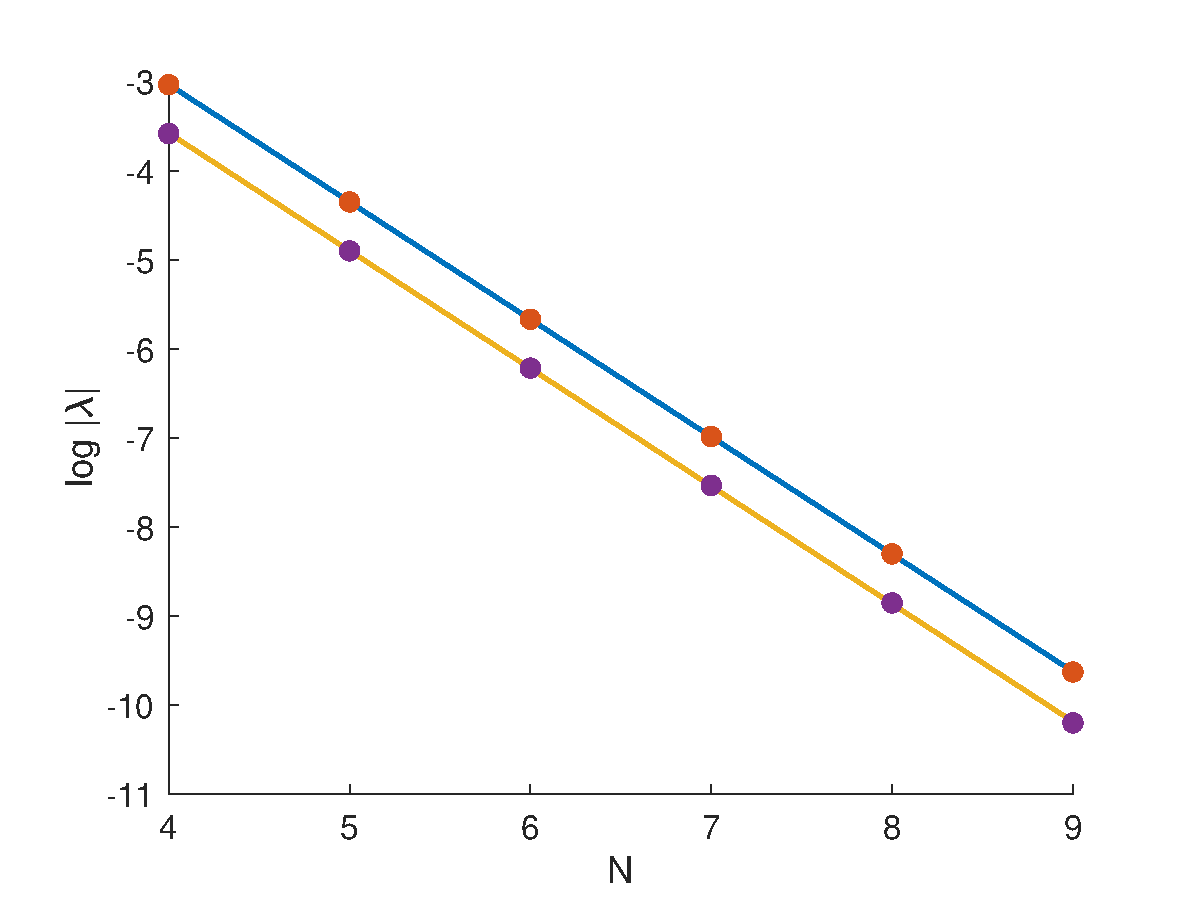
\includegraphics[width=5cm]{images/other/dnlsPPPdecay.eps}
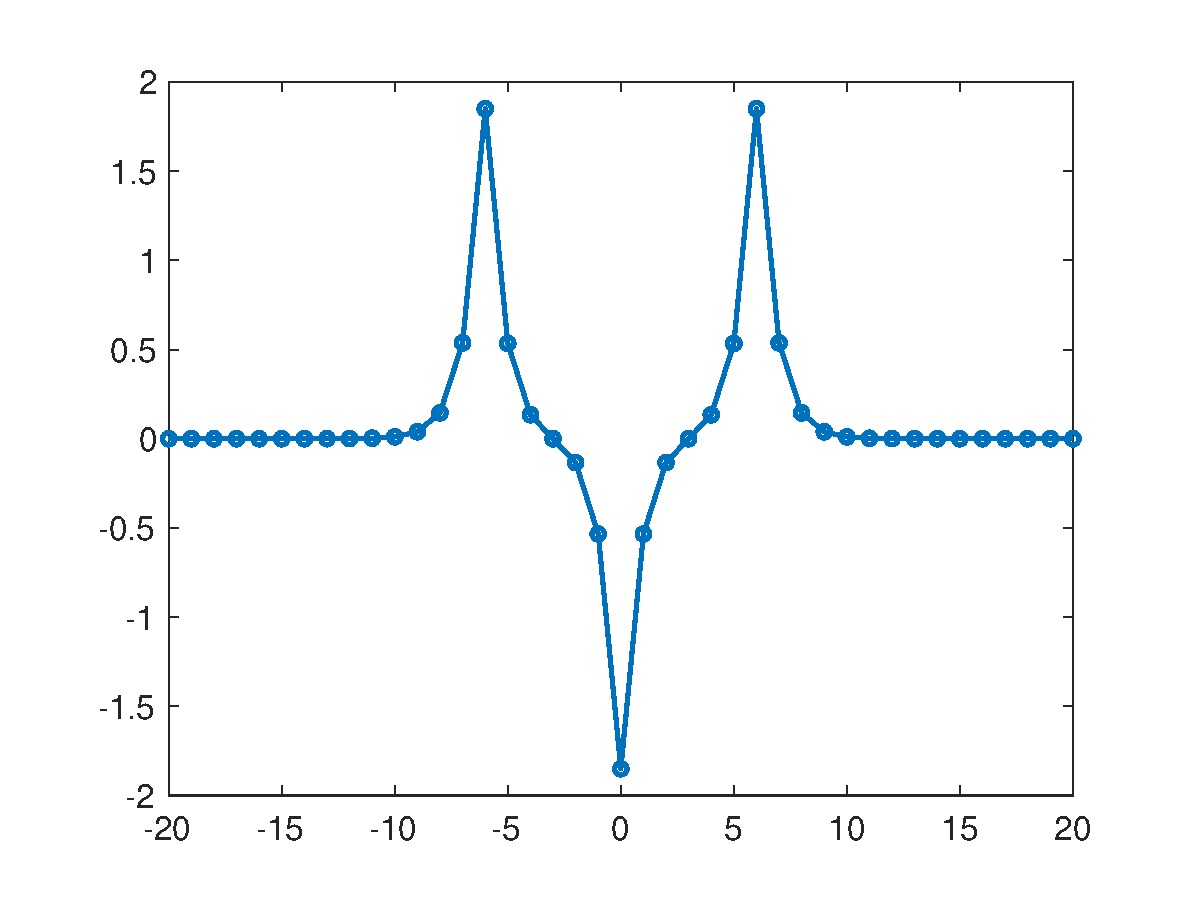
\includegraphics[width=5cm]{images/other/dnlsPMP.eps}
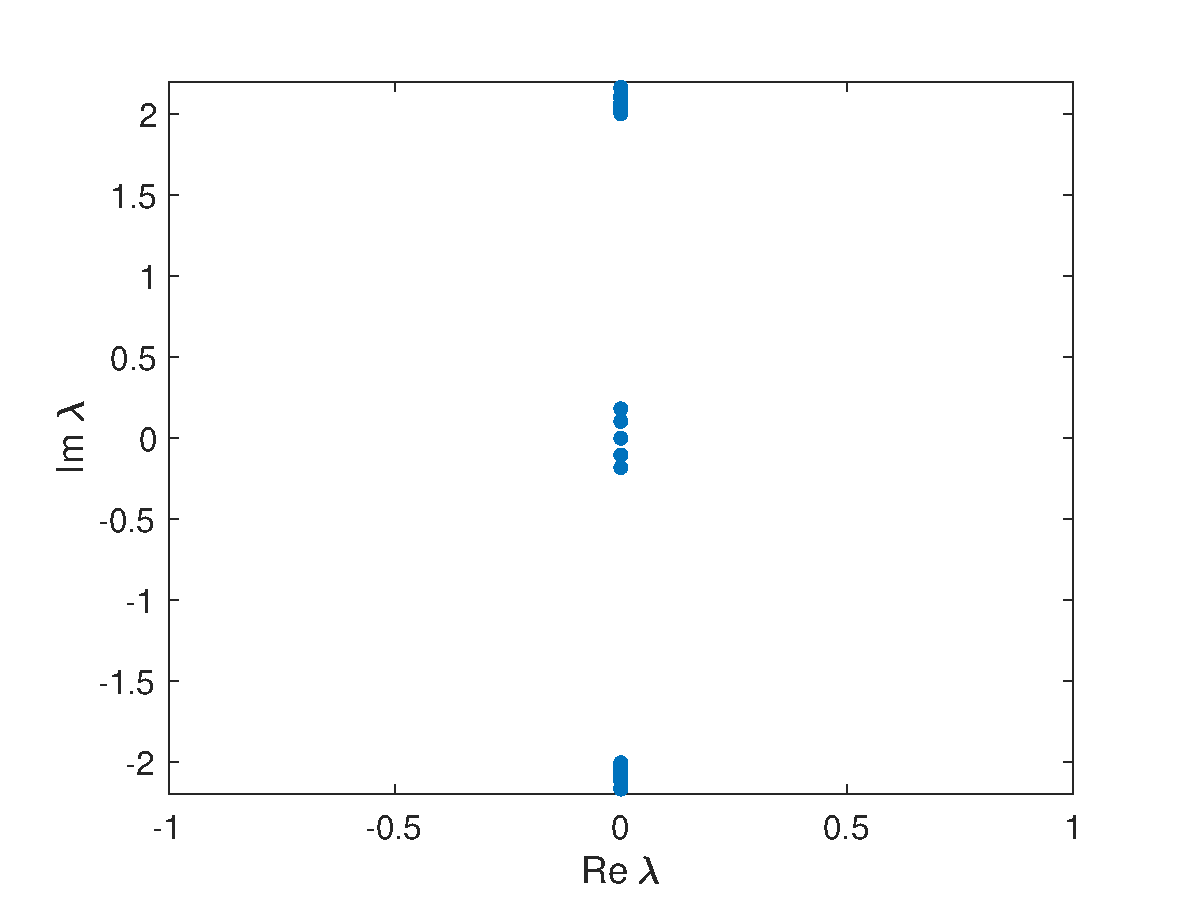
\includegraphics[width=5cm]{images/other/dnlsPMPeig.eps}
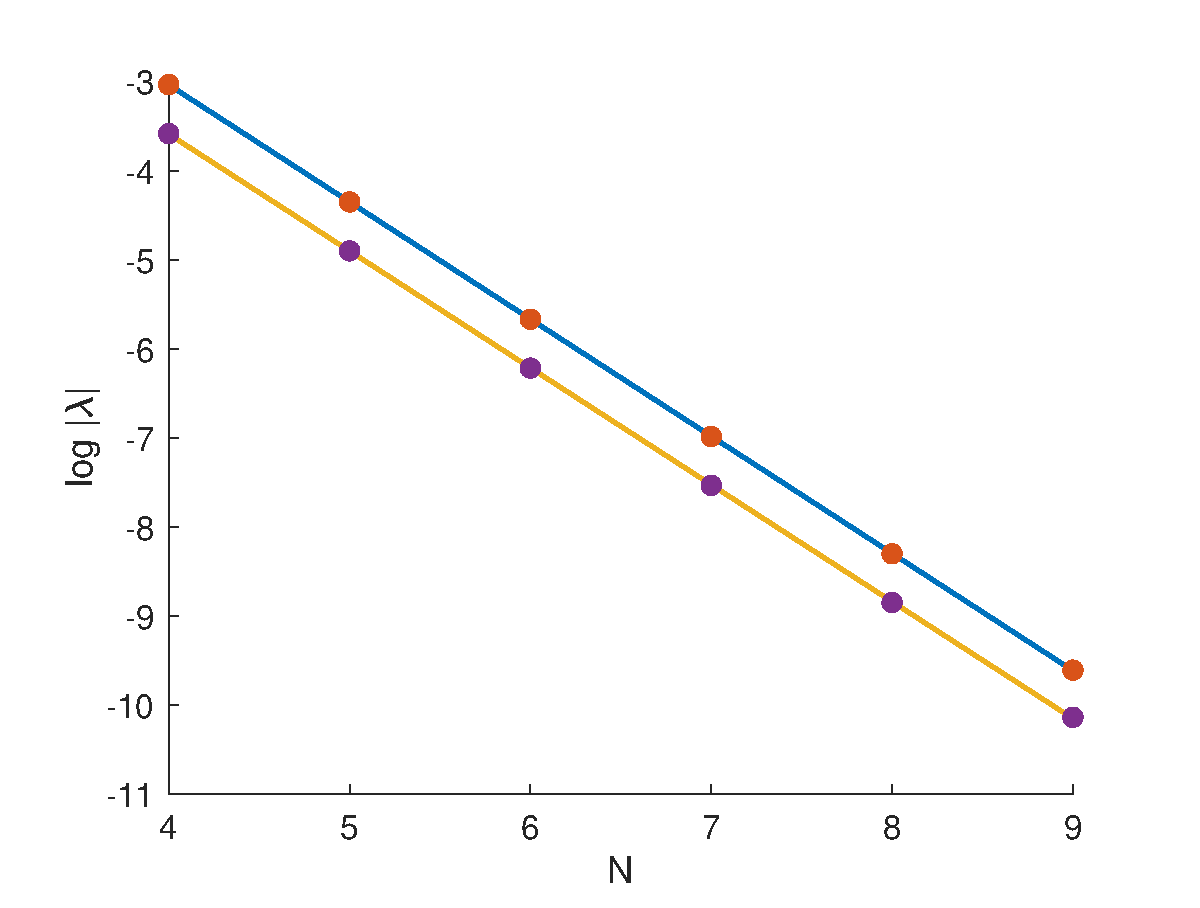
\includegraphics[width=5cm]{images/other/dnlsPMPdecay.eps}
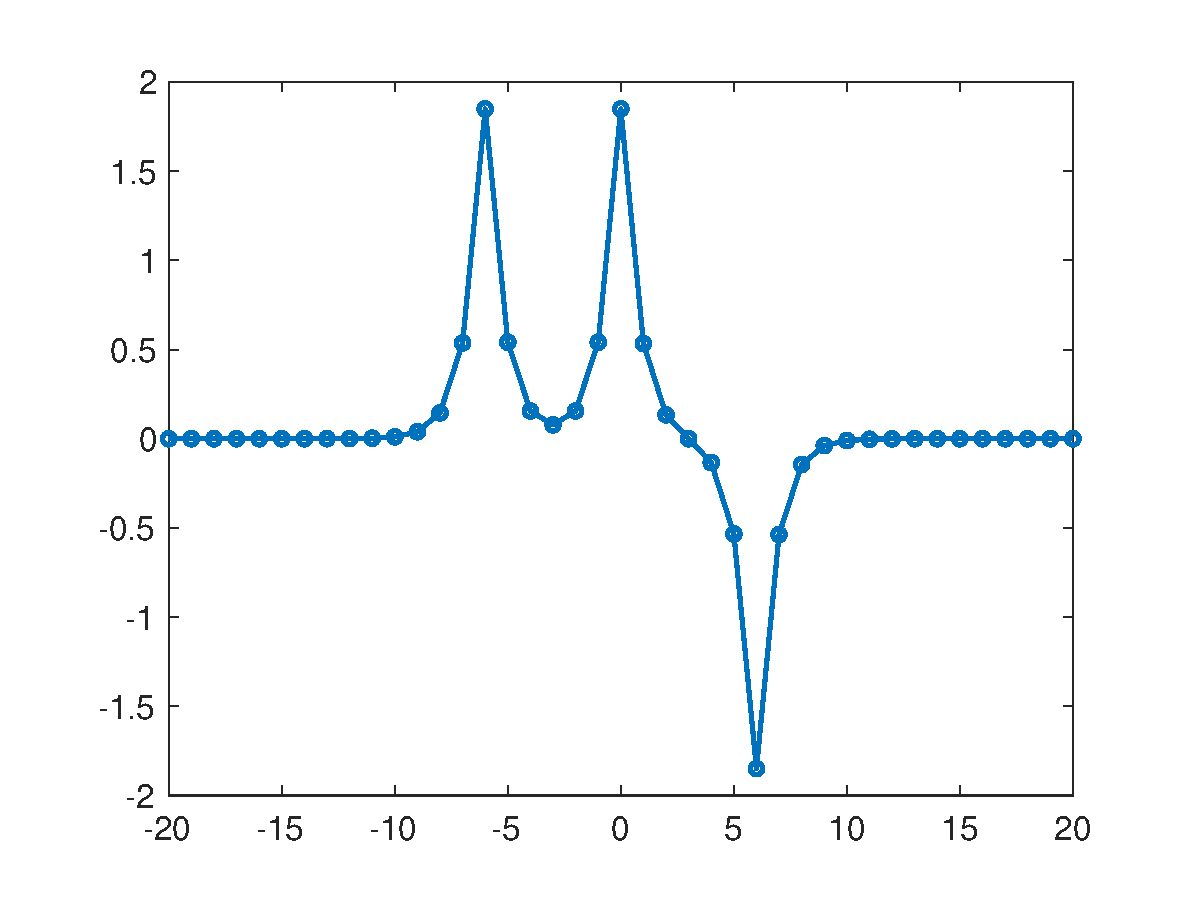
\includegraphics[width=5cm]{images/other/dnlsPPM.eps}
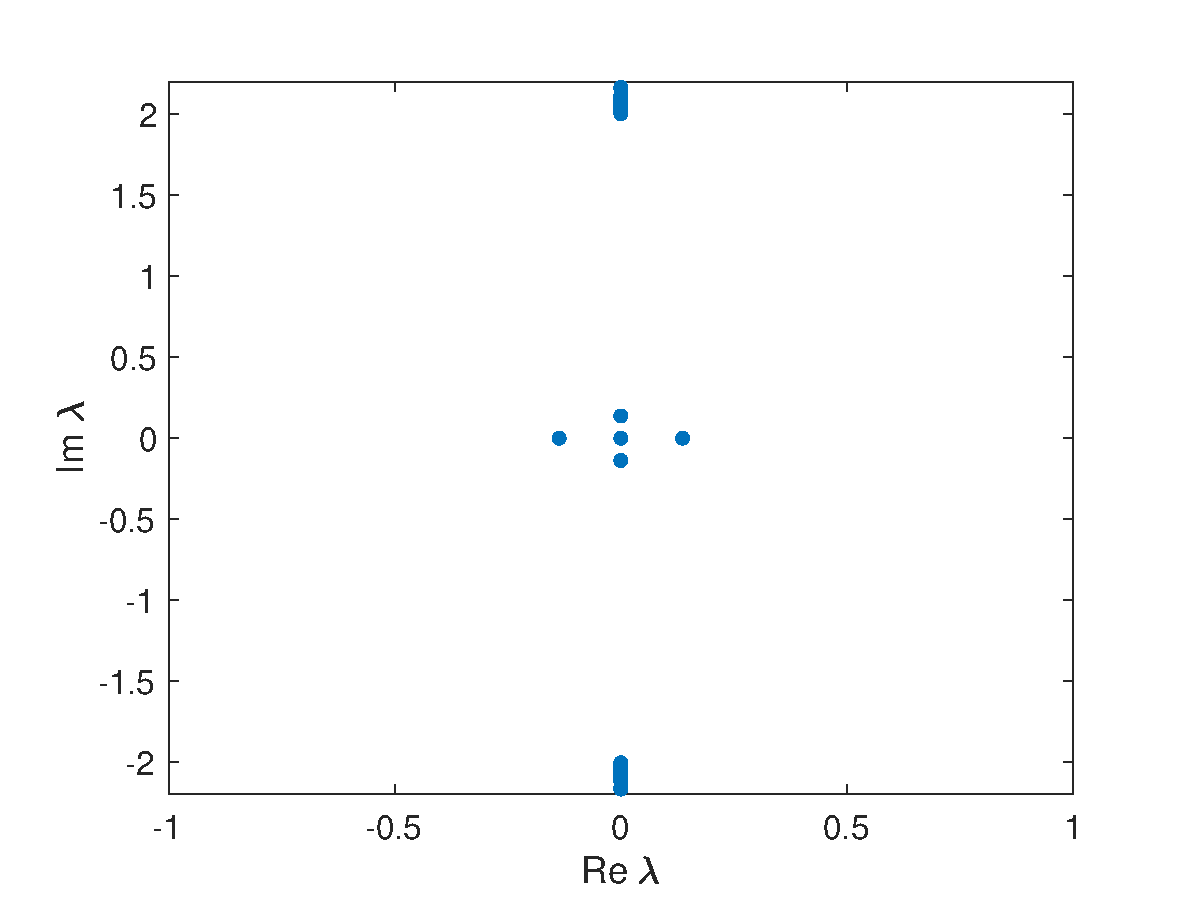
\includegraphics[width=5cm]{images/other/dnlsPPMeig.eps}
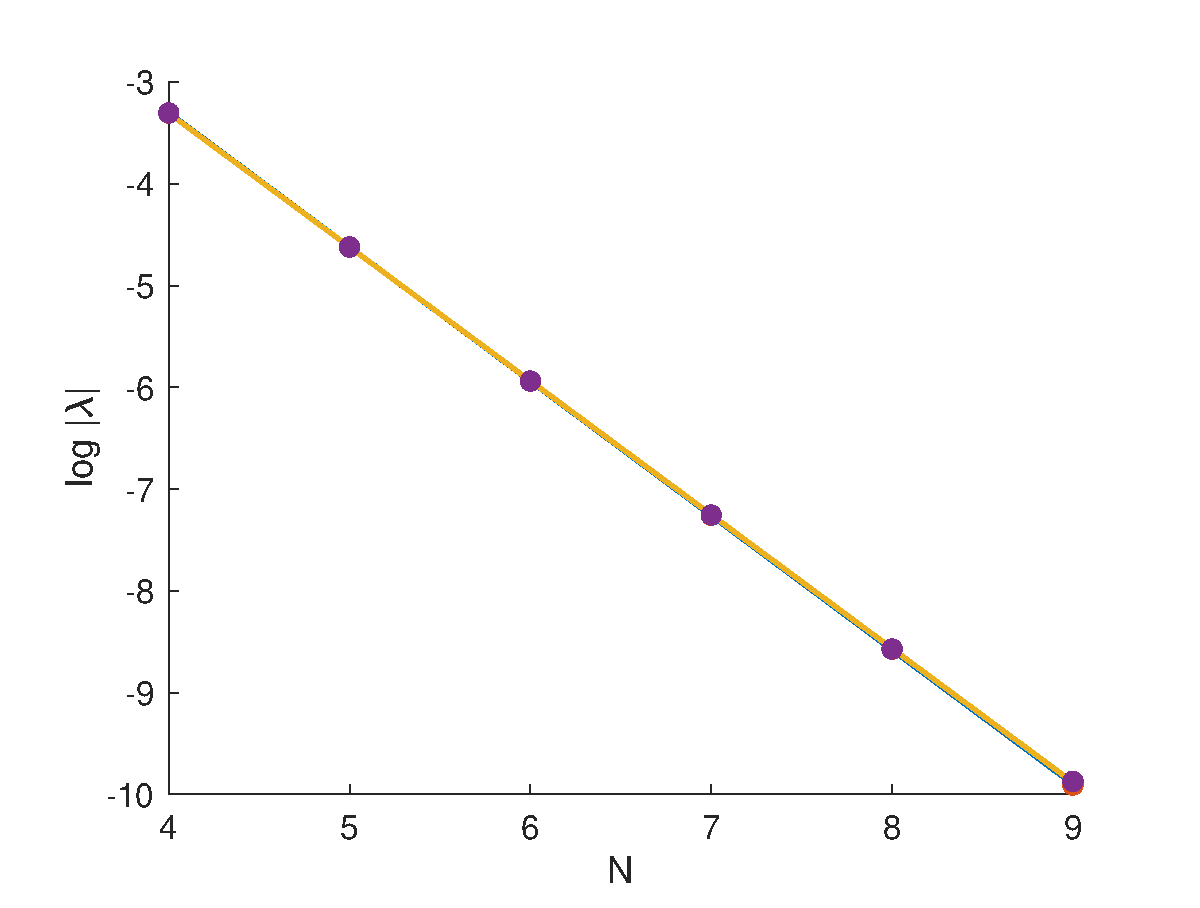
\includegraphics[width=5cm]{images/other/dnlsPPMdecay.eps}
\caption[Solutions and eigenvalue patterns for triple pulses in DNLS]{Solution profile (left panel), spectral plane eigenvalue pattern (center panel), and plot of $\log(\lambda)$ vs. $N$ with least squares linear regression line (right panel) for the three triple pulse cases: $+++$ (top), $+-+$ (middle), and $++-$ pulses. Parameters $\omega = 2$ and $d = 1.0$.}
\label{fig:eigendecay2}
\end{figure}

We can also look at triple pulses with unequal pulse distances $N_1$ and $N_2$. If $N_1 < N_2 < 2 N_1$, then by \cref{DNLSeigcorr2}, there are two pairs of eigenvalues of order $r^{-N_1/2}$ and $r^{-N_2/2}$. We can similarly verify these decay rates numerically.

Finally, we can compute the leading order term in equation \cref{eigsDNLS} and compare that to the numerical result. A value for $\omega$ is chosen, and the single pulse solution $q(n; \omega)$ is constructed numerically using parameter continuation from the anti-continuum limit until the desired coupling parameter $d$ is reached. The terms $b_i$ from the matrix $A$ are computed by using equation \cref{bieq} with the numerically constructed solution $q(n; \omega)$. For the derivative $\partial_\omega q(n; \omega)$, solutions $q(n; \omega + \epsilon)$ and $q(n; \omega - \epsilon)$ are constructed numerically for small $\epsilon$ by parameter continuation from the anti-continuum limit to the same value of $d$. The derivative $\partial_\omega q(n; \omega)$ is computed from these via a centered finite difference method; this is used together with $q(n; \omega)$ to calculate the Melnikov sum $M$. 

First, we consider the case of equal pulse distances. We use the expressions from \cref{DNLSeigcorr} to compute the leading order term for the interaction eigenvalues, and we compare this to the results from Matlab's \texttt{eig} function. In \cref{fig:error1} we fix the inter-pulse distances and plot the log of the relative error of the eigenvalues versus the coupling parameter $d$. For intermediate values of $d$, the relative error is less than $10^{-3}$. Since the stability results are not uniform in $d$, i.e. they hold for sufficiently large $N$ once $d$ and $\omega$ are chosen, we do not expect to have a nice relationship between the error and $d$. This is furthermore complicated by the fact that additional sources of error arise from  
numerically approximating $b_i$ and $M$. In principle, though, the method (and the asymptotic prediction) yields
satisfactory results except for the vicinity of the 
anti-continuum limit (where the notion of the single
pulse is highly discrete) and the near-continuum limit
(where the role of discreteness is too weak). 
It is interesting to point out that at a ``middle
ground'' between these two limits, namely around $d=0.5$,
we observe the optimal performance of the theoretical
prediction. 

\begin{figure}
\centering
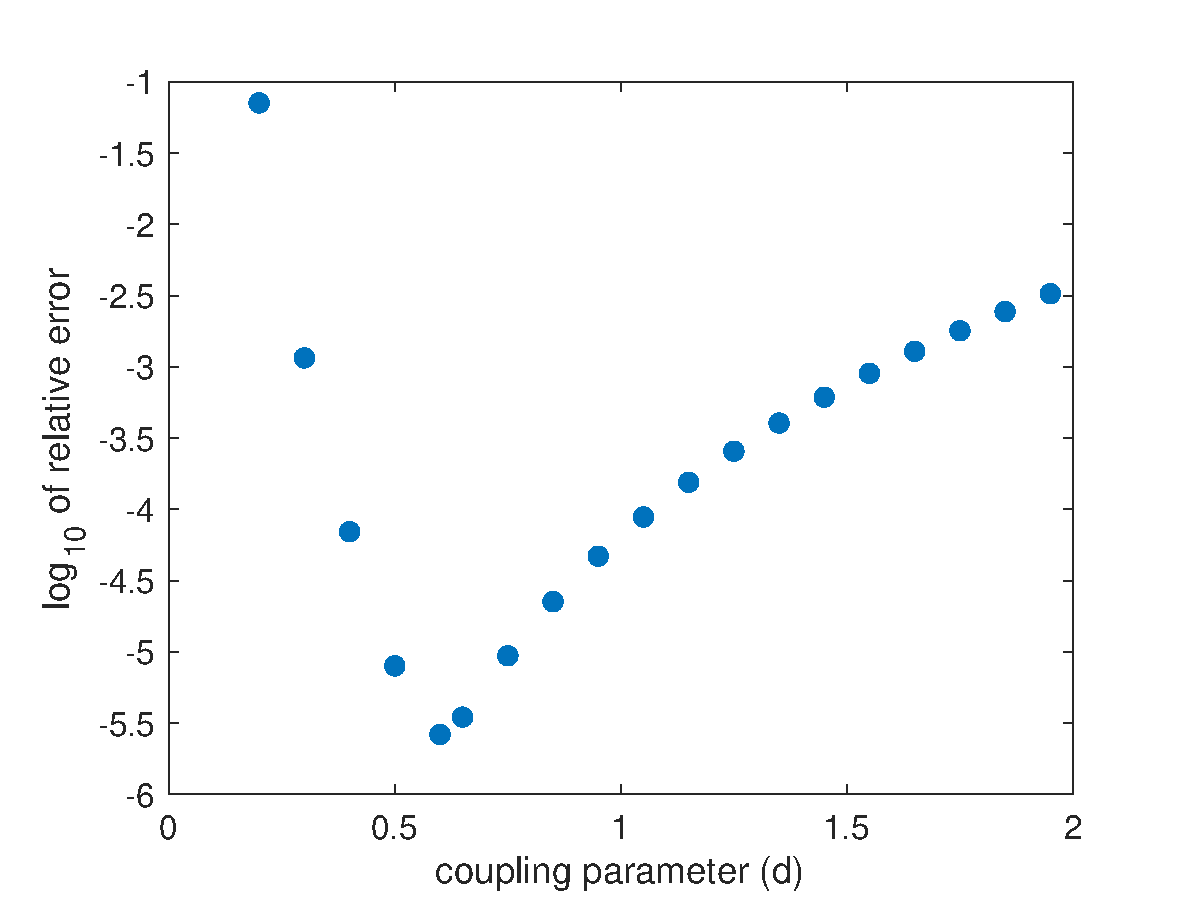
\includegraphics[width=7cm]{images/other/errors1.eps}
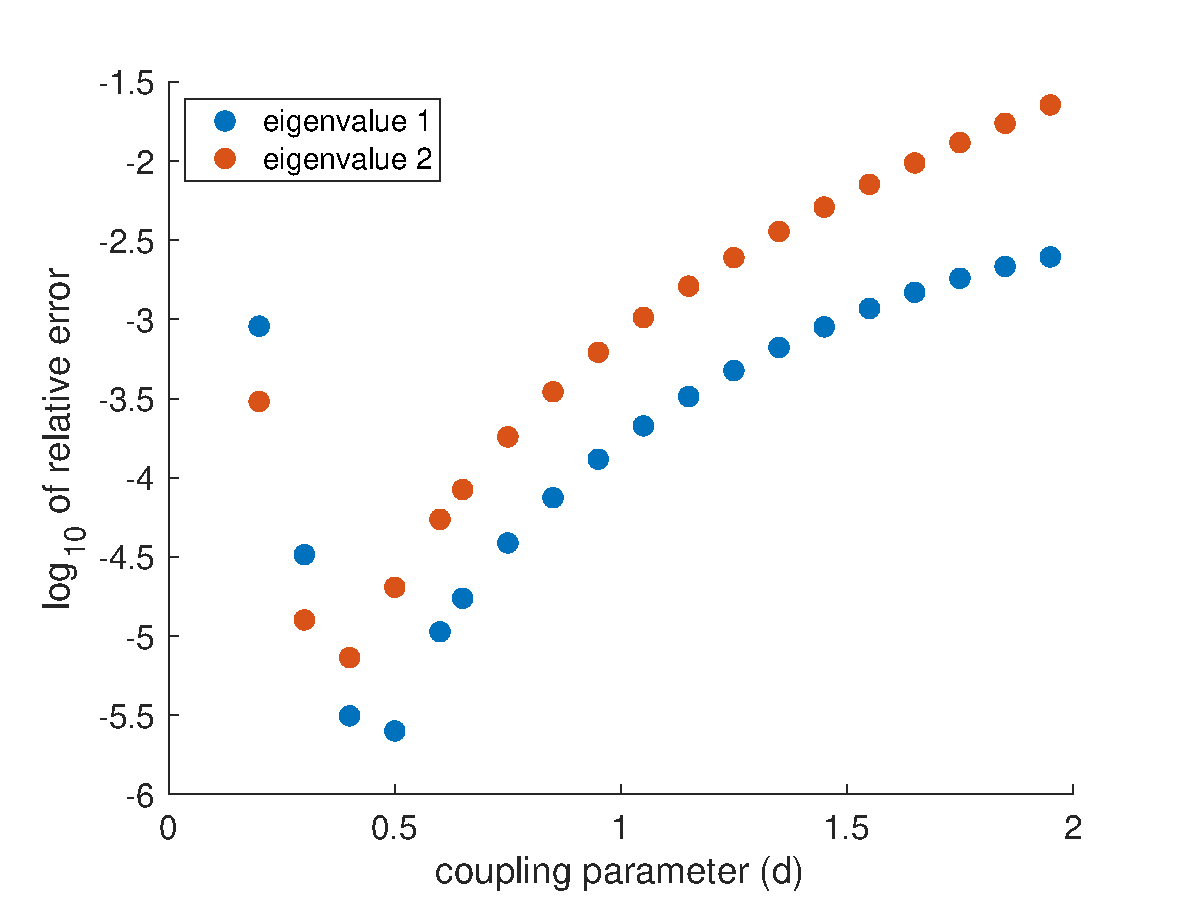
\includegraphics[width=7cm]{images/other/errors2.eps}
\caption[Error plot for eigenvalue computations for symmeteric multi-pulses in DNLS]{Log of relative error of eigenvalues vs. coupling parameter $d$ for double (in phase) 
pulse $++$ ($N_1 = 10$) and triple (out-of-phase) pulse $+-+$ ($N_1 = N_2 = 8)$. $\omega = 2$ in both cases.}
\label{fig:error1}
\end{figure}

We can also do this for triple pulses with unequal pulse distances. In this case, we use \cref{DNLSeigcorr2} to compute the eigenvalues to leading order. \cref{fig:error2} shows the log of the relative error of the eigenvalues versus the coupling parameter $d$.
For intermediate values of $d$, the relative error is again less than $10^{-3}$. Once again this validates the relevance
of the method especially so for the case of 
intermediate ranges of the coupling parameter $d$.

\begin{figure}
\centering
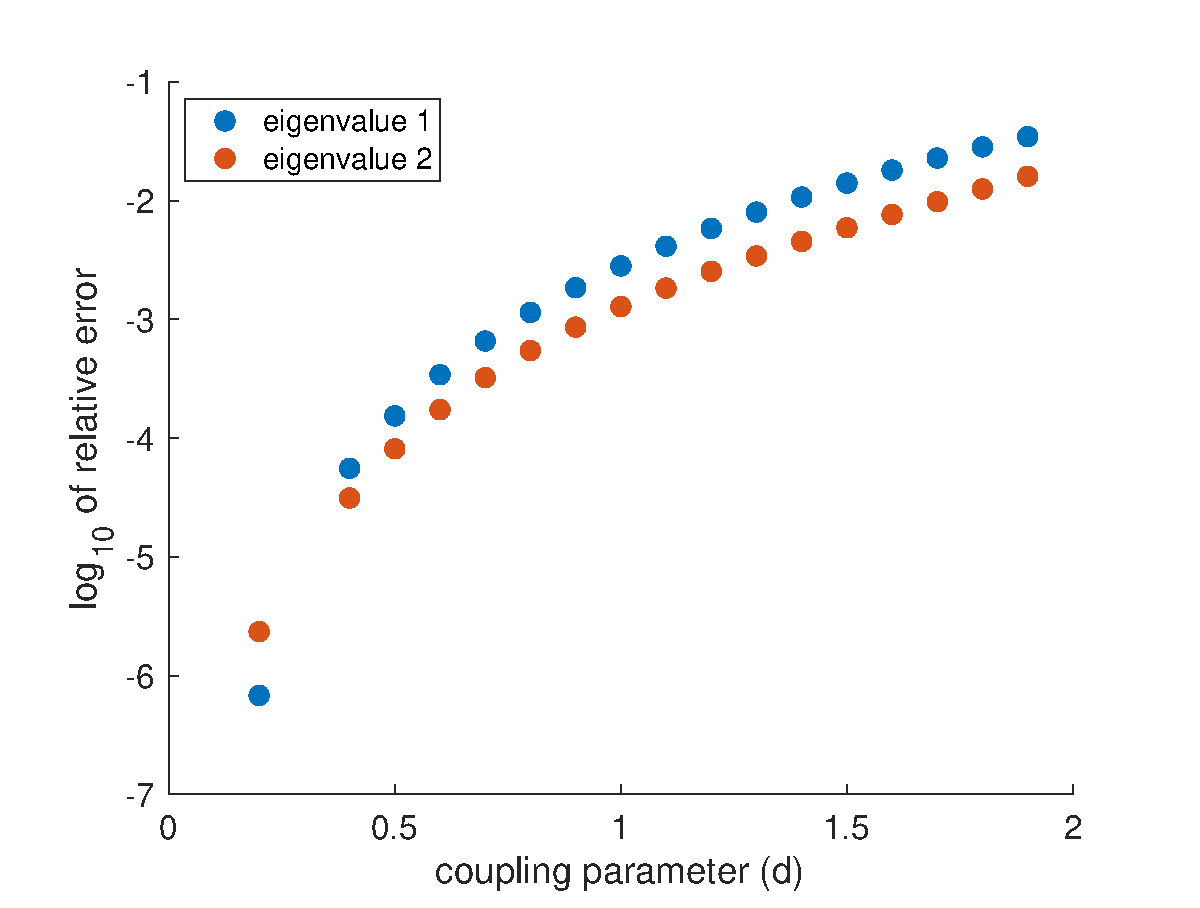
\includegraphics[width=7cm]{images/other/errors3.eps}
\caption[Error plot for eigenvalue computations for asymmetric multi-pulses in DNLS]{Log of relative error of eigenvalues vs. coupling parameter $d$ for triple in-phase pulse $+++$ with unequal pulse distances ($N_1 = 8, N_2 = 6$), $\omega = 2$.}
\label{fig:error2}
\end{figure}

\iffulldocument\else
	\bibliographystyle{amsalpha}
	\bibliography{thesis.bib}
\fi

\end{document}